% =============================================================================
% RUL Evaluation Protocol Study: Springer JIM submission
% =============================================================================
\documentclass[pdflatex,sn-basic,NameDate]{sn-jnl}

\usepackage{graphicx}%
\usepackage{amsmath,amssymb,amsfonts}%
\usepackage{booktabs}%
\usepackage{multirow}%
\usepackage{float}%
\usepackage{bm}%
\usepackage{indentfirst}%

\hyphenpenalty=10000
\exhyphenpenalty=10000
\emergencystretch=3em
\setlength{\parindent}{2em}

\graphicspath{{figures/}}

\begin{document}

\title[Reliability Audit for Data-Driven Predictive Maintenance]{An Evaluation-Protocol Audit Framework for Data-Driven Bearing Remaining Useful Life Prediction}

\author*[1]{\fnm{Zhongkuan} \sur{Ma}\kern0.3em}\email{2024212760@nefu.edu.cn}
\affil[1]{\orgname{~Northeast Forestry University, }\orgaddress{\city{Harbin}, \country{China}}}


\abstract{\hspace*{2em}An RUL benchmark score is interpretable only when the evaluation protocol matches the deployment setting. We formalize an empirically grounded evaluation-protocol audit template for bearing remaining useful life (RUL) prediction and apply it through a $2 \times 2$ protocol comparison of label construction and split strategy, plus a history-construction intervention. Across three public datasets, replacing dense overlapping history construction with non-overlapping stride-10 construction lowered random-split $R^2$ and raised RMSE and MAE in all deep-model cells. The linear-regression baseline was unchanged because it uses single-window features rather than history sequences. The piecewise-random protocol still produced higher mean $R^2$ than the trajectory-normalized linear-LOOCV reference, but the separation was dataset-dependent. We interpret random splitting as a different task (within-trajectory interpolation) rather than as an invalid protocol. The STAR reporting template packages these findings as a reporting/audit checklist for authors, reviewers, and reliability teams.}

\keywords{Predictive maintenance, Reliability assessment, Bearing RUL prediction, Evaluation protocol, Temporal splitting, Reproducibility}

\maketitle

\section{Introduction}
Bearing failures are a common cause of downtime in rotating machinery, and RUL predictions are used to decide when to intervene \citep{lei2018machinery,zhao2019deep}. In deployment, RUL models decide when maintenance should occur, so their predictions need to be trustworthy enough to support that decision. For industrial model selection, the relevant question is whether a reported score supports decisions for a new asset. The same principle may apply to changed operating conditions or different machine stations, but we do not evaluate those settings here. Deep learning methods have reported high $R^2$ values on public bearing datasets \citep{rul_lstm_uq_2022,reg_lstm_2021,gru_tim_2021,transformer_tim_2023}. A common benchmark protocol family combines piecewise linear labels with an 80\% plateau, random sequence-level splitting of non-overlapping history sequences, and sliding historical input sequences across the full life trajectory. Protocols adopted in laboratory benchmarks may not match the information constraints of real deployment.
In practical manufacturing systems, RUL models are expected to generalize across different assets rather than interpolate previously observed degradation trajectories. These choices define different prediction tasks, not just formatting details. A piecewise label with an 80\% plateau holds most of a trajectory at one target value, which turns much of the regression into a transition-detection problem. A random sequence-level split can put temporally adjacent samples from the same bearing on both sides of the training/test boundary, making the test task an interpolation on a trajectory the model has already seen. When historical input sequences are also constructed with stride~1, train and test can share large portions of their input windows. We compare stride~1 with non-overlapping stride~10 sequences under otherwise fixed preprocessing, models, labels, and seeds. Because this comparison also changes sequence count and temporal sampling density, we interpret it as a history-construction intervention rather than as an isolated estimate of overlap alone.


We contribute:
\begin{enumerate}
    \item an empirically grounded evaluation-protocol audit template for bearing RUL benchmarks, formalized through problem definition, protocol operators, and reporting checks;
    \item a controlled intervention comparing overlapping (stride~1) and non-overlapping (stride~10) history construction under random sequence-level splitting, with cross-bearing LOOCV as the held-out-bearing reference, on XJTU-SY, PHM2012, and IMS;
    \item per-fold results, 95\% confidence intervals, bounded effect sizes, RMSE, and MAE for all model-dataset combinations;
    \item evidence that replacing dense overlapping history construction with non-overlapping stride-10 sequences reduces random-split scores of sequence-based RUL models when history construction is changed;
    \item random split-ratio and chronological time-block sensitivity analysis under non-overlapping sequences;
    \item a reusable STAR reporting template with continuous labels, per-bearing holdout, constant baselines, and multi-model reporting, designed as the reporting output of the experiments.
\end{enumerate}
Random splitting is not universally invalid; this study quantifies how history-window construction, label construction, and split strategy jointly change reliability estimates, with an interaction whose direction and magnitude vary across datasets and models.


\section{Motivating Protocol Choices}
Recent bearing RUL benchmark studies often use a protocol family that combines piecewise linear labels with an 80\% plateau and random sequence-level splitting. We do not claim that every paper using this family is unreliable. We test whether these choices change the reliability estimate under controlled conditions on three public datasets, with the claims remaining auditable through the reported results and reproducibility package rather than through an audit of individual publications.

A quantitative prevalence count is not feasible because many surveyed papers omit methods or code. We therefore treat the protocol family as a potential source of optimistic estimates rather than as evidence about specific studies. A controlled comparison on public data is a more direct test of protocol sensitivity because the same preprocessing, models, seeds, and metrics are used for every protocol. Differences in $R^2$ should therefore be interpreted as protocol sensitivity under the fixed conditions of this study rather than as implementation-specific differences.

\section{Related Work}
Bearing RUL prediction has moved from physics-based degradation models \citep{paris1963critical,kotzalas2004fatigue,li2022physics} to data-driven models built on CNNs \citep{ince2016real}, recurrent networks, and transformers \citep{rul_lstm_uq_2022,reg_lstm_2021,transformer_tim_2023}. Much of this literature concentrates on architecture design. Evaluation protocols receive less attention, and reviews note the absence of standardized benchmarks \citep{zhao2021deep,caesarendra2021machine}. These reviews mainly catalogue models and features; they identify evaluation inconsistency as a limitation without providing a concrete protocol or an audit checklist. This paper addresses that gap by developing an empirically grounded evaluation-protocol audit template, quantifying label and split effects under controlled protocols, and translating the findings into the STAR checklist. The contribution is a reusable audit procedure, not a new architecture.

Recent PHM and time-series methodology work has emphasized benchmark transparency, uncertainty reporting, and reproducibility controls \citep{phmconf2025rethinking,review2020bearing,mst2024cqr,icsrs2023splitconformal,phme2026conformal,ress2022bayesian,eaai2025explainable}; a smaller subset addresses data leakage and evaluation audits \citep{leakage_nature,leakage_frontiers}. These studies note that reported accuracy depends on preprocessing, label construction, split design, uncertainty reporting, and reproducibility controls. Our contribution is an empirically grounded evaluation-protocol audit template that combines a controlled history-window intervention with a $2\times 2$ protocol comparison of label and split effects on three bearing datasets and four model families, plus a concrete STAR reporting template that turns this evidence into an auditable deployment checklist.

Label construction is usually treated as fixed preprocessing, but it changes the difficulty of the target. A plateau at the start of life compresses most of the label distribution into a single value. The effect of this compression depends on the dataset and the split, which is why label and split should be evaluated jointly rather than in isolation.

Recent time-series and ecological studies distinguish direct sample leakage from within-trajectory dependence \citep{leakage_nature,leakage_frontiers}. Random splitting does not necessarily copy identical samples into training and test, but it places dependent samples from the same trajectory on both sides of the split. With stride~1 history construction, adjacent sequences also share most of their input windows, adding input-level overlap beyond ordinary trajectory dependence. We compare stride~1 with non-overlapping stride~10 sequences as a history-construction intervention. Because this comparison also changes sequence count and temporal sampling density, it should not be treated as a pure overlap-only manipulation.

The methodological gap is whether reported scores measure prediction for new bearings, interpolation within the same bearing, or interpolation aided by overlapping input windows, and whether the piecewise plateau label amplifies that gap. We measure these effects on the same preprocessing, models, seeds, and metrics, which is a bearing-RUL-specific question beyond the generic warning that time-series samples should not be shuffled.

We do not classify individual papers from metadata. In many studies, the split and label details are not reported at a level that allows reliable classification from metadata or abstracts, and a table built from incomplete information would introduce the same reproducibility problem this paper addresses. The protocol choices used here are instead grounded in the two practices discussed in the cited RUL and time-series evaluation literature. Appendix A illustrates how the STAR checklist can be used for transparent reporting extraction without classifying studies as valid or invalid.

\subsection{Evaluation Protocols in Prognostics}
Time-series evaluation protocols differ in what they ask a model to do. A random sequence-level split keeps samples from the same trajectory on both sides of the training/test boundary. The test task then becomes interpolation on a trajectory the model has already observed. A chronological split keeps the same bearing in training but asks the model to extrapolate into later degradation stages. A grouped-by-bearing split removes the test bearing from training and therefore provides a held-out-bearing reference under the available benchmark datasets, subject to the trajectory-normalized labels used in this study. These protocols are not interchangeable, and reported performance cannot be compared across them without specifying which task was used.

Bearing run-to-failure signals add another complication. Consecutive windows are strongly autocorrelated, and the degradation process is monotonic in most cases. A model trained on randomly assigned sequences from the same bearing can memorize the trajectory shape and use nearby temporal context to interpolate test samples. That behavior is useful for tracking a known degradation process, but it is not evidence that the model can predict the behavior of a new bearing under a different load or operating condition.

The same issue appears in other time-series domains, where direct sample leakage is distinguished from dependence-induced interpolation \citep{leakage_nature,leakage_frontiers}. For bearing RUL, the practical consequence is that benchmark scores should be interpreted as properties of the joint choice of label, split, and history-window construction, not as standalone properties of the model. The STAR checklist proposed later makes this dependency explicit.

\section{Methodology}
\begin{figure}[t]
\centering
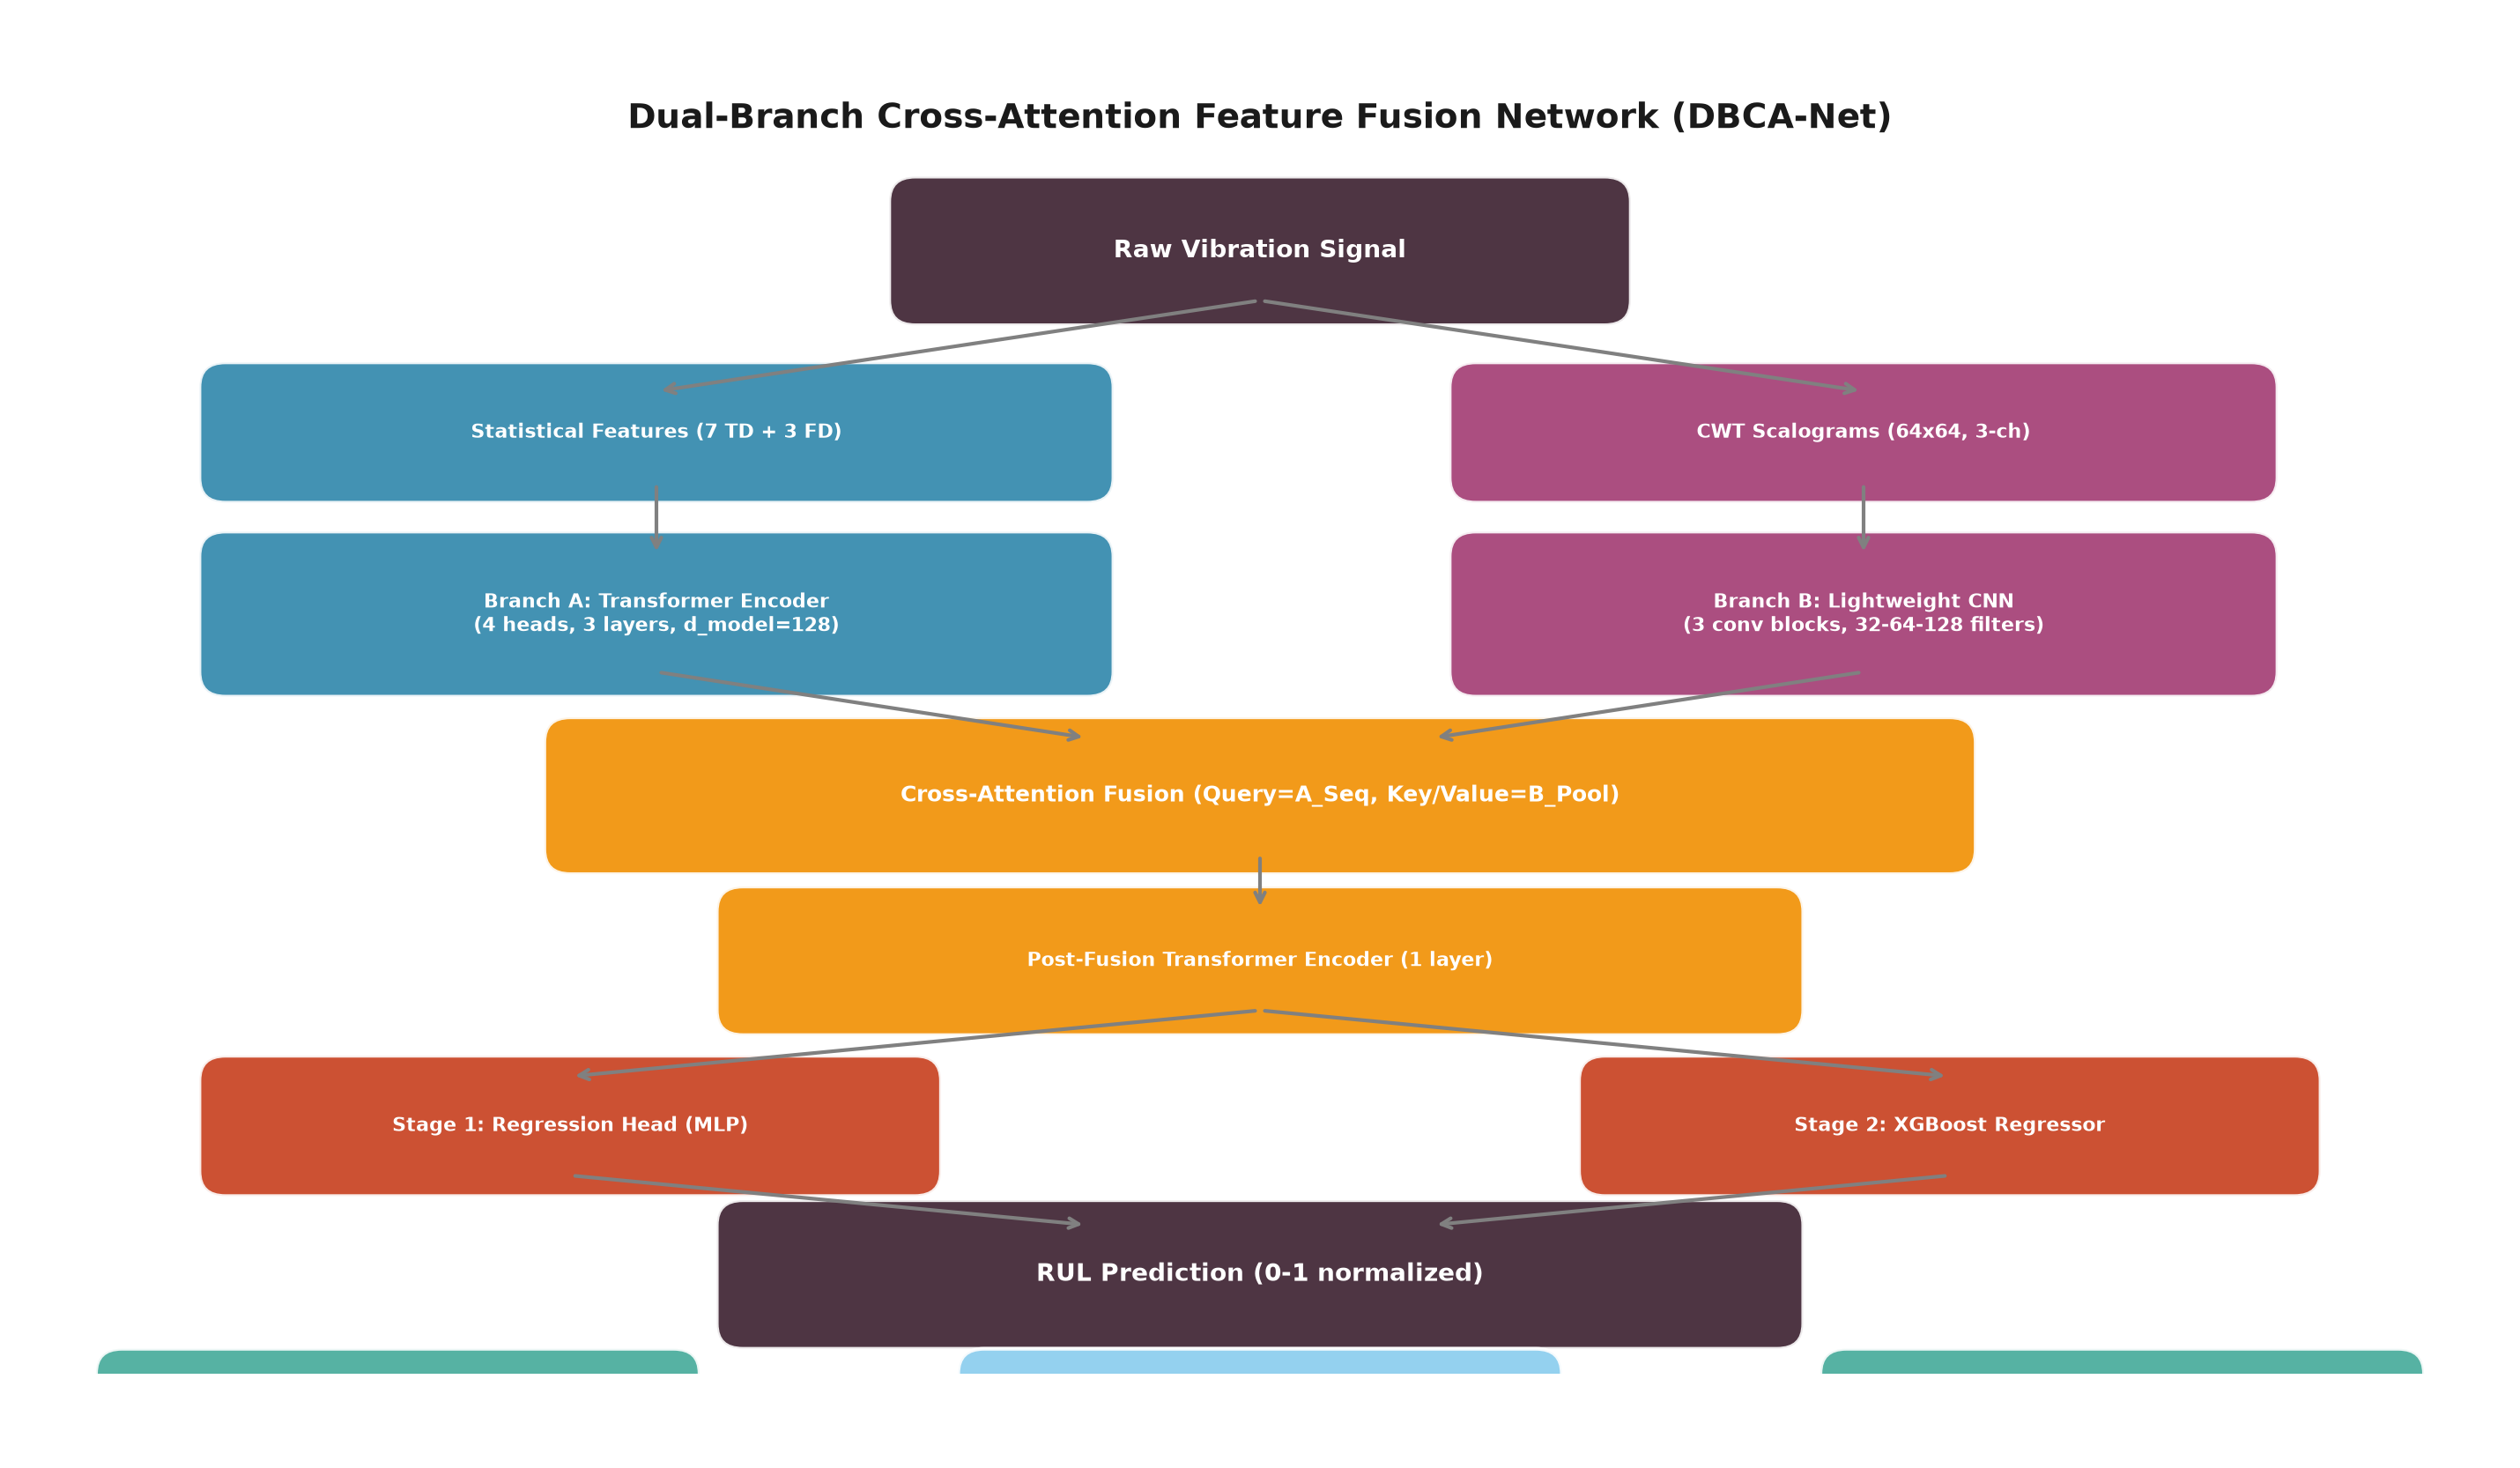
\includegraphics[width=0.95\textwidth]{figures/fig_overview.png}
\caption{Overview of the evaluation-protocol study: from bearing trajectories to feature windows, history sequences, labels, split protocols, and reliability metrics.}
\label{fig:overview}
\end{figure}

\subsection{Problem Formulation and Notation}

Let $\mathcal{B}$ denote the set of run-to-failure bearings and let $W_i=\{x_{i,1},\ldots,x_{i,T_i}\}$ denote the feature trajectory of bearing $i$, where $x_{i,t}\in\mathbb{R}^{10}$ is the ten-dimensional statistical and spectral feature vector extracted from the $t$-th non-overlapping vibration window and $T_i$ is the trajectory length. For history length $L=10$ and stride $s$, the history sequence ending at time $t$ is
\begin{equation}
H_{i,t}^{(s)} = \left[x_{i,t-(L-1)s}, x_{i,t-(L-2)s}, \ldots, x_{i,t}\right]^\top,
\label{eq:history}
\end{equation}
where valid sequences are formed for $t\geq (L-1)s+1$. The primary non-overlapping construction uses $s=L$; the overlapping reference construction uses $s=1$.

The normalized RUL label is defined by the linear target
\begin{equation}
y_{i,t}^{\mathrm{lin}} = 1 - \frac{t}{T_i},
\label{eq:y_lin}
\end{equation}
or the piecewise plateau target
\begin{equation}
y_{i,t}^{\mathrm{pw}} =
\begin{cases}
1.0, & t < 0.8T_i,\\
\dfrac{T_i-t}{0.2T_i}, & t \geq 0.8T_i.
\end{cases}
\label{eq:y_pw}
\end{equation}
Given a model $f_\theta$ and an evaluation protocol $\mathcal{P}$, the task is to estimate $\hat y_{i,t}=f_\theta(H_{i,t}^{(s)})$ from training data $\mathcal{D}_{\mathrm{tr}}(\mathcal{P})$ and evaluate it on held-out data $\mathcal{D}_{\mathrm{te}}(\mathcal{P})$. The protocol determines whether $\mathcal{D}_{\mathrm{tr}}$ and $\mathcal{D}_{\mathrm{te}}$ contain windows from the same bearing and whether adjacent history sequences can share input windows.

Table~\ref{tab:notation_rul} summarizes the notation used throughout the paper.

\begin{table*}[t]
\centering
\caption{Notation used in the problem formulation, evaluation protocols, and reporting metrics.}
\label{tab:notation_rul}
\small
\resizebox{\textwidth}{!}{%
\begin{tabular}{@{}lll@{}}
\toprule
\textbf{Symbol} & \textbf{Description} & \textbf{Unit} \\
\midrule
$\mathcal{B}$ & Set of run-to-failure bearings & --- \\
$W_i$ & Feature trajectory of bearing $i$ & --- \\
$x_{i,t}$ & Ten-dimensional feature vector at time $t$ & --- \\
$T_i$ & Length of trajectory $i$ in windows & windows \\
$L$ & History length & windows \\
$s$ & History stride & windows \\
$H_{i,t}^{(s)}$ & History sequence for bearing $i$, time $t$, stride $s$ & --- \\
$y_{i,t}$ & Normalized RUL label & --- \\
$\hat y_{i,t}$ & Predicted normalized RUL & --- \\
$\mathcal{P}$ & Evaluation protocol & --- \\
$\mathcal{D}_{\mathrm{tr}},\mathcal{D}_{\mathrm{va}},\mathcal{D}_{\mathrm{te}}$ & Training, validation, and test sets & --- \\
\bottomrule
\end{tabular}}
\end{table*}

\subsection{Datasets}
We use three public run-to-failure datasets:
\begin{itemize}
    \item \textbf{XJTU-SY} \citep{xjtusy2019dataset}: the predefined eight-bearing reproducibility subset (Bearing1\_1 through Bearing1\_5 and Bearing2\_1 through Bearing2\_3) from conditions 1 and 2, yielding 15,928 windows. Condition 3 and Bearing2\_4--Bearing2\_5 were not included in this fixed subset, so all reported XJTU-SY results remain exactly consistent with the archived preprocessing and convergence artifacts.
    \item \textbf{PHM2012} \citep{nectoux2012pronostia}: 6 learning-set bearings, yielding 7,534 windows.
    \item \textbf{IMS} \citep{ims2006}: 3 run-to-failure test sets (first, second, and fourth), yielding 75,712 windows.
\end{itemize}
The PU dataset is a benchmark for fault classification rather than full run-to-failure RUL trajectories, so it is not used for RUL label generation. Each vibration signal is segmented into non-overlapping windows of 2,560 samples; the stride therefore equals the window length. Ten statistical and spectral features are extracted per window. For a window $x_1,\dots,x_n$, the time-domain features are
\begin{align}
\mathrm{F}_{\mathrm{rms}} &= \sqrt{\frac{1}{n}\sum_{i=1}^{n}x_i^2}, &
\mathrm{F}_{\mathrm{mean}} &= \frac{1}{n}\sum_{i=1}^{n}x_i, \nonumber \\
\mathrm{F}_{\mathrm{var}} &= \frac{1}{n-1}\sum_{i=1}^{n}(x_i-\mathrm{F}_{\mathrm{mean}})^2, &
\mathrm{F}_{\mathrm{kurt}} &= \frac{\frac{1}{n}\sum_{i=1}^{n}(x_i-\mathrm{F}_{\mathrm{mean}})^4}{\left[\frac{1}{n}\sum_{i=1}^{n}(x_i-\mathrm{F}_{\mathrm{mean}})^2\right]^2}, \nonumber \\
\mathrm{F}_{\mathrm{skew}} &= \frac{\frac{1}{n}\sum_{i=1}^{n}(x_i-\mathrm{F}_{\mathrm{mean}})^3}{\left[\frac{1}{n}\sum_{i=1}^{n}(x_i-\mathrm{F}_{\mathrm{mean}})^2\right]^{3/2}}, &
\mathrm{F}_{\mathrm{crest}} &= \frac{\max_i |x_i|}{\mathrm{F}_{\mathrm{rms}}}, \nonumber \\
\mathrm{F}_{\mathrm{pp}} &= \max_i x_i - \min_i x_i. \nonumber
\end{align}
With $X_k=\sum_{i=1}^{n}x_i e^{-2\pi j (i-1)(k-1)/n}$, $P_k=|X_k|^2$, and $p_k=P_k/\sum_l P_l$, the spectral features are
\begin{align}
\mathrm{F}_{\mathrm{dom}} &= \arg\max_k |X_k|, &
\mathrm{F}_{\mathrm{energy}} &= \sum_k P_k, &
\mathrm{F}_{\mathrm{entropy}} &= -\sum_k p_k \log_2 p_k. \nonumber
\end{align}
A history length of 10 windows is used for LSTM, TCN, and PatchTST inputs. The primary sequence construction uses a non-overlapping stride of 10 windows, so no two history sequences share an input window. We also report a stride~1 sliding-sequence protocol as the overlapping reference. History sequences are constructed within each bearing before splitting; cross-bearing LOOCV leaves the test bearing out of training and validation by construction. Feature normalization parameters are estimated from the training split only and applied to validation and test splits.

RUL labels are normalized to the $[0,1]$ range within each trajectory. This removes differences in absolute life span across datasets and keeps the regression target comparable. Normalization is applied as a deterministic monotonic scaling of RUL and does not place any test sample in training. It does, however, assume end-of-life information when constructing the target, which is a deployment constraint; we retain it here for comparability across datasets and models. Relative RUL normalization is an offline benchmark construction choice; we do not treat it as an online deployment procedure. A separate incremental-normalization control was not added in this paper because it would change the regression target and require a second preprocessing and training pipeline, which would reduce comparability with the standard benchmark target used across the public datasets. We disclose this assumption and leave incremental normalization for future work. PHM2012 is used with its six learning-set bearings because the public challenge test set does not provide ground-truth RUL for supervised cross-validation.

\subsection{Labels and Evaluation Protocols}
We compare two label families:
\begin{equation}
\text{RUL}_{\text{lin}}(t) = 1 - t/T,
\label{eq:linear}
\end{equation}
\begin{equation}
\text{RUL}_{\text{pw}}(t) =
\begin{cases}
1.0, & t < 0.8T \\
(T - t)/(0.2T), & t \geq 0.8T.
\end{cases}
\label{eq:piecewise}
\end{equation}

\begin{figure}[t]
\centering
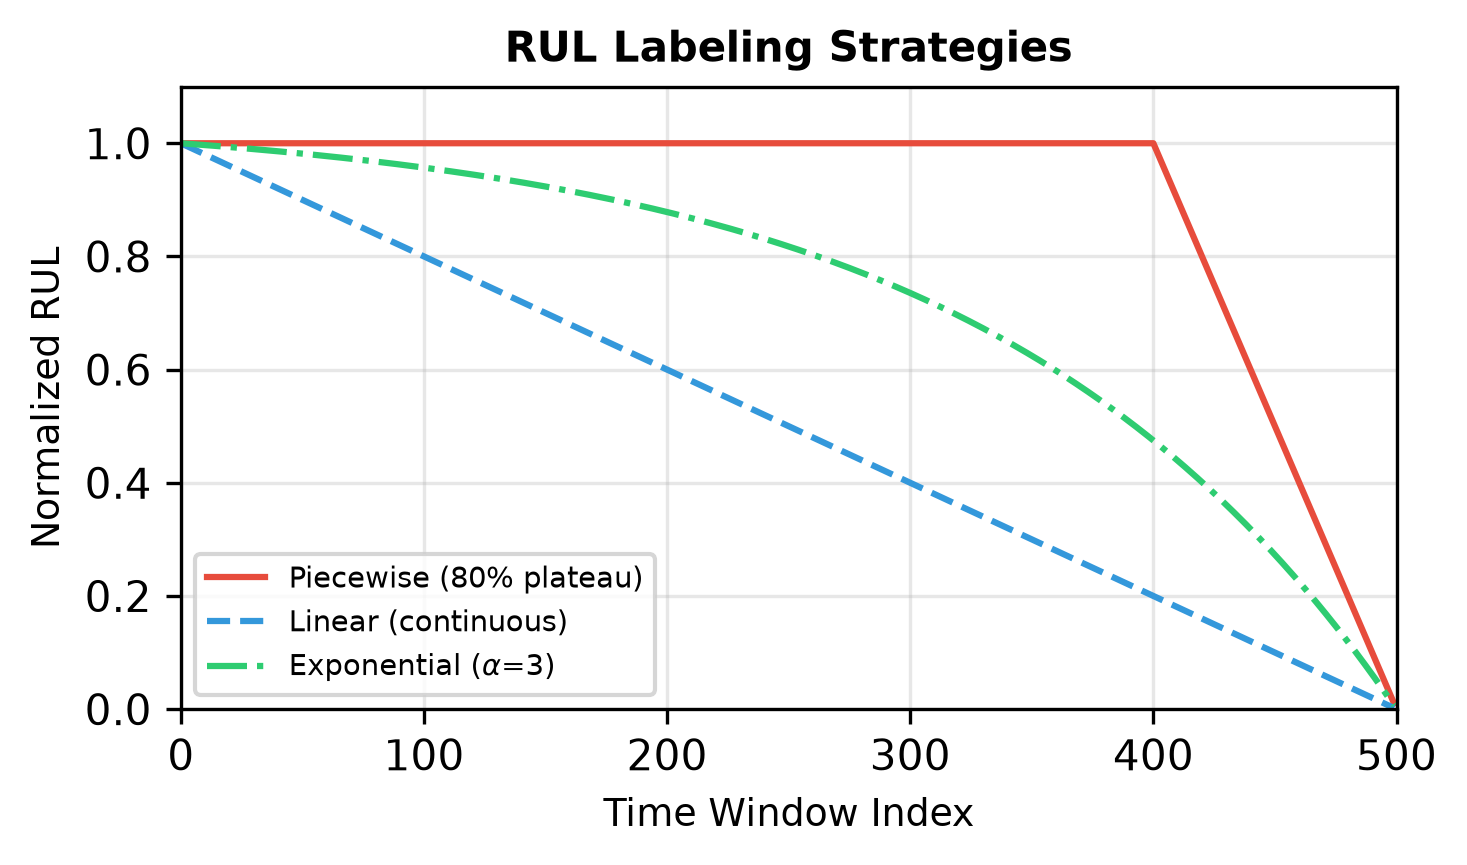
\includegraphics[width=0.9\textwidth]{figures/fig_labeling_strategies.png}
\caption{Comparison of linear and piecewise plateau RUL label construction.}
\label{fig:labels}
\end{figure}

The primary cross-bearing evaluation protocol uses non-overlapping history sequences (stride~10), linear labels, and leave-one-bearing-out cross-validation (LOOCV). For each test bearing, one other bearing is used for validation, and the remaining bearings are used for training. The validation bearing is the next bearing in the dataset order, with a cyclic offset: for the last bearing in the dataset order, validation cycles back to the first bearing. This choice is deterministic, does not use test labels, and avoids random validation selection; the fixed ordering is disclosed so that a reader can audit the results. The fixed rule should therefore be regarded as a deterministic control choice rather than a universally optimal validation strategy. The random-split protocol uses piecewise labels with a 70\%/15\%/15\% random sequence-level split of all non-overlapping history sequences, again with stride~10 history construction. All non-overlapping history sequences from the available bearings are pooled and randomly divided into training, validation, and test sets at a 70\%/15\%/15\% ratio. The stride~1 sliding-sequence construction is retained as the overlapping reference protocol. The $2\times2$ protocol comparison concerns label construction and split strategy; stride is a separate history-construction intervention and is not treated as a third factor in the descriptive interaction analysis.

Let $\mathcal{D}_i$ be the set of history sequences constructed from bearing $i$. The three protocols are then defined as:
\begin{align}
\mathcal{P}_{\mathrm{LOOCV}}:&\quad
\mathcal{D}_{\mathrm{tr}}=\bigcup_{j\notin\{k,v\}}\mathcal{D}_j,\quad
\mathcal{D}_{\mathrm{va}}=\mathcal{D}_v,\quad
\mathcal{D}_{\mathrm{te}}=\mathcal{D}_k,\\
\mathcal{P}_{\mathrm{random}}:&\quad
\mathcal{D}=\bigcup_{i\in\mathcal{B}}\mathcal{D}_i \ \text{partitioned into}
70\%/15\%/15\%\ \text{train/validation/test},\\
\mathcal{P}_{\mathrm{chrono}}:&\quad
\mathcal{D}_{i,\mathrm{tr}}:\mathcal{D}_{i,\mathrm{va}}:\mathcal{D}_{i,\mathrm{te}}
=70:15:15\ \text{for each bearing}\ i,
\label{eq:protocols}
\end{align}
where $k$ is the test bearing and $v$ is the deterministic validation bearing for $\mathcal{P}_{\mathrm{LOOCV}}$.

\begin{figure}[t]
\centering
\fbox{\parbox{0.95\textwidth}{%
\small
\textbf{LOOCV:} train on bearings A and B, validate on bearing C, test on bearing D. No window from D appears in training or validation.\\
\textbf{Random split:} all windows from A, B, C, and D are pooled and randomly divided into train, validation, and test sets. Non-overlapping stride~10 history sequences are used for the primary protocol; stride~1 overlapping sequences are retained as the reference.\\
\textbf{Chronological split:} for each bearing, the first 70\% of non-overlapping history sequences are used for training, the next 15\% for validation, and the last 15\% for testing.
}}
\caption{Comparison of the three evaluation protocols under non-overlapping history-sequence construction. The overlapping stride~1 construction is used only as the reference intervention.}
\label{fig:protocols}
\end{figure}

\subsection{Evaluation Audit Checks}
The audit checks evaluate whether a reported bearing RUL benchmark can support a deployment-oriented decision. They consist of five checks: task definition, split integrity, target integrity, anchor baseline, and reporting completeness. Task definition requires the intended use case to be stated as either trajectory tracking or held-out-bearing generalization under the benchmark data. Split integrity requires the test-bearing windows to be absent from training and validation when held-out-bearing generalization is claimed. Target integrity requires the label construction and plateau parameters to be explicit. Anchor baseline requires a constant predictor floor. Reporting completeness requires per-fold or per-seed results together with $R^2$, RMSE, MAE, and confidence or range summaries. The controlled experiments in this paper operationalize these checks by holding preprocessing, models, seeds, and metrics fixed while changing only the protocol dimensions under audit.

\subsection{Models and Training}
We use four learned model classes:
\begin{itemize}
    \item \textbf{Linear Regression} on the 10 extracted features;
    \item \textbf{LSTM}: two-layer LSTM with 128 hidden units;
    \item \textbf{TCN}: dilated temporal convolutional network with channel widths $32 \to 64 \to 128$.
    \item \textbf{PatchTST} \citep{patchtst2023}: patch-based time-series transformer with patch length 4, stride 2, embedding dimension 64, four attention heads, and three encoder layers, drawing on the Transformer architecture \citep{vaswani2017attention}.
\end{itemize}
A constant predictor baseline, which always outputs the mean training RUL, is reported as the reference floor.

The models are simple by design. We do not rank architectures; we test whether protocol effects persist across model families. Keeping the models simple helps isolate protocol effects instead of model engineering. CNN-based models are not included because this study focuses on protocol sensitivity rather than architecture ranking. The selected classes cover linear, recurrent, convolutional temporal, and transformer-based inductive biases.

All neural models are trained with MSE loss, AdamW (learning rate $10^{-3}$, weight decay $10^{-5}$), cosine annealing, batch size 1024, and early stopping with patience 30. TCN uses dropout $0.2$ and PatchTST uses dropout $0.1$. XJTU-SY and PHM2012 use a maximum of 100 epochs; IMS uses a maximum of 60 epochs because of its much larger size. Model initialization and random-split permutation are controlled by fixed seeds, and the best validation epoch is recorded for every run. The mean best epochs range from 2 to 97 across model-dataset combinations, confirming that the protocol allows convergence or early-stopping where cross-bearing generalization fails. All neural runs in the archived results were executed on an NVIDIA GeForce RTX 4060 Laptop GPU (8 GB) with PyTorch; individual model-dataset cells converged within several minutes, and complete dataset sweeps required tens of minutes.

\subsection{Statistical Reporting}
All metrics are computed at the sample level on the test split used by each protocol. For $n$ test samples with observed labels $y_j$ and predictions $\hat y_j$, the reporting metrics are
\begin{equation}
R^2 = 1 - \frac{\sum_{j=1}^{n}(y_j-\hat y_j)^2}{\sum_{j=1}^{n}(y_j-\bar y)^2},
\label{eq:r2}
\end{equation}
\begin{equation}
\mathrm{RMSE} = \sqrt{\frac{1}{n}\sum_{j=1}^{n}(y_j-\hat y_j)^2},
\label{eq:rmse}
\end{equation}
\begin{equation}
\mathrm{MAE} = \frac{1}{n}\sum_{j=1}^{n}|y_j-\hat y_j|,
\label{eq:mae}
\end{equation}
where $\bar y$ is the mean observed label in the test split. $R^2$ is the coefficient of determination; RMSE and MAE are computed on trajectory-normalized RUL and are therefore unitless fractions of the normalized trajectory length.
As in the benchmark preprocessing, predicted normalized RUL values are clipped to $[0,1]$ before metric computation. We disclose this because clipping can reduce reported error when a model overshoots the target scale.
For LOOCV, we report the mean $R^2$, standard deviation, and 95\% confidence interval computed with Student's $t$-distribution across held-out bearings. The CI reflects between-bearing fold variance, not sample-level prediction variance. Per-fold values are stored in the reproducibility artifacts. Main-table LOOCV and random-split summaries, and the per-fold/per-seed values in Appendix~B, are computed from the same designated converged runs stored in the reproducibility package. The validation-bearing sensitivity analysis is reported in Section~5.5 as a separate converged sensitivity run; it is not an alternative main-table estimate.

On XJTU-SY, the held-out bearings are similar in window count and degradation structure, and each fold uses six training bearings, with the test and validation bearings rotating by a fixed offset. Fold-level $R^2$ is therefore highly consistent and the CI is narrow. On IMS, only three test sets exist, so the CI is wide. XJTU-SY and PHM2012 provide the primary statistical evidence, while IMS provides consistent directional evidence rather than a precise estimate.

Random splitting is repeated with eight fixed seeds (42--49) for every dataset and model, and we report the mean and the observed min--max range. Seed-level repetitions are treated as repeated computational runs rather than independent physical samples, so they are not used to construct population-level hypothesis tests. Effect sizes are reported with Cliff's delta as a descriptive stability summary. Seed-level bootstrap intervals for the random-split means are reported in Table~\ref{tab:random_bootstrap_nonoverlap}; these intervals quantify computational split sensitivity rather than bearing-level uncertainty.
\begin{equation}
\delta = \Pr(x_i > y_j) - \Pr(x_i < y_j),
\label{eq:cliff}
\end{equation}
where the probabilities are empirical frequencies over all ordered pairs of observations, and ties do not contribute to either term. Cliff's delta is bounded in $[-1, 1]$ and avoids the distortion of Cohen's $d$ when fold-level variance is tiny. Under non-overlapping sequence construction, complete separation between piecewise random runs and linear-LOOCV folds is not universal. IMS retains Cliff's delta $=1.0$ for all three deep models; PHM2012 ranges from $0.458$ to $0.917$; XJTU-SY is $0.500$ for all three deep models. We do not report permutation $p$-values because LOOCV folds and random seeds are not exchangeable experimental units. Delta is used as a descriptive effect-size summary rather than a population-level treatment effect. To summarize the four-cell design, we also report a descriptive interaction term: $\Delta_{\mathrm{interaction}} = (R^2_{\mathrm{pw,random}} - R^2_{\mathrm{pw,LOOCV}}) - (R^2_{\mathrm{lin,random}} - R^2_{\mathrm{lin,LOOCV}})$. This term summarizes whether the label and split effects are additive in mean $R^2$; it is not used as a significance test.

\subsection{Split Sensitivity Analysis}
To check whether the random-split result depends on the specific 70/15/15 ratio, we add two additional random ratios with TCN and piecewise labels:
\begin{itemize}
    \item 60\%/20\%/20\%;
    \item 80\%/10\%/10\%.
\end{itemize}
We also implement a chronological time-block split at 70\%/15\%/15\%: each bearing trajectory is split by time, with the first 70\% of non-overlapping history sequences used for training, the next 15\% for validation, and the final 15\% for testing. This removes random interleaving while still training on the same bearing as the test set. Chronological evaluation also involves temporal extrapolation and degradation-stage imbalance, so the negative $R^2$ values should be interpreted as a combination of these factors rather than as a pure leakage measurement.

\section{Results}
\subsection{Effect of Non-Overlapping History Construction}
We first examine the history-construction intervention. Replacing stride~1 with stride~10 sequences reduced random-split $R^2$ in all 18 deep-model cells (LSTM, TCN, and PatchTST across three datasets and two label families), while RMSE and MAE increased in all 18 cells. The decreases range from $0.080$ on XJTU-SY to $0.419$ on PHM2012, with PHM2012 showing the largest changes and IMS showing highly consistent decreases of about $0.19$--$0.21$. The linear-regression baseline was unchanged because it uses single-window features rather than history sequences, so the stride intervention does not alter its input construction. Table~\ref{tab:stride_random} reports the paired $R^2$, RMSE, and MAE comparison for every deep-model cell. In the archived preprocessing used here, every test sequence under the stride~1 random-split cells shared at least one input window with training across all eight seeds and all three datasets; under stride~10 construction, this input-level overlap rate is zero. The main implication is that dense overlapping history construction can produce higher random-split scores, reflecting a different within-trajectory interpolation task rather than demonstrating held-out-bearing quality. Because the intervention also changes sequence count and temporal sampling density, the size of the gap should not be read as overlap alone.

\begin{table*}[!ht]
\centering
\caption{Random-split history-construction comparison (stride=1 versus stride=10). Values are mean $R^2$, RMSE, and MAE across eight seeds (42--49); $\Delta R^2$ is the stride=10 value minus the stride=1 value. RMSE and MAE are computed on trajectory-normalized RUL.}
\label{tab:stride_random}
\small
\resizebox{\textwidth}{!}{%
\begin{tabular}{lllccccccc}
\toprule
Dataset & Label & Model & $R^2_{\mathrm{stride}=1}$ & $R^2_{\mathrm{stride}=10}$ & $\Delta R^2$ & $\mathrm{RMSE}_{\mathrm{stride}=1}$ & $\mathrm{RMSE}_{\mathrm{stride}=10}$ & $\mathrm{MAE}_{\mathrm{stride}=1}$ & $\mathrm{MAE}_{\mathrm{stride}=10}$ \\
\midrule
\midrule
XJTU-SY & Linear & LSTM & 0.223 & 0.117 & -0.106 & 0.254 & 0.267 & 0.243 & 0.254 \\
XJTU-SY & Linear & TCN & 0.218 & 0.124 & -0.094 & 0.255 & 0.266 & 0.243 & 0.253 \\
XJTU-SY & Linear & PatchTST & 0.203 & 0.095 & -0.108 & 0.257 & 0.271 & 0.245 & 0.255 \\
XJTU-SY & Piecewise & LSTM & 0.410 & 0.310 & -0.100 & 0.181 & 0.190 & 0.100 & 0.108 \\
XJTU-SY & Piecewise & TCN & 0.410 & 0.330 & -0.080 & 0.181 & 0.187 & 0.106 & 0.115 \\
XJTU-SY & Piecewise & PatchTST & 0.416 & 0.314 & -0.101 & 0.181 & 0.189 & 0.101 & 0.108 \\
\midrule
PHM2012 & Linear & LSTM & 0.794 & 0.455 & -0.338 & 0.131 & 0.215 & 0.090 & 0.171 \\
PHM2012 & Linear & TCN & 0.826 & 0.557 & -0.270 & 0.121 & 0.194 & 0.082 & 0.145 \\
PHM2012 & Linear & PatchTST & 0.793 & 0.616 & -0.177 & 0.131 & 0.180 & 0.091 & 0.137 \\
PHM2012 & Piecewise & LSTM & 0.785 & 0.518 & -0.266 & 0.108 & 0.168 & 0.053 & 0.096 \\
PHM2012 & Piecewise & TCN & 0.843 & 0.424 & -0.419 & 0.092 & 0.186 & 0.047 & 0.117 \\
PHM2012 & Piecewise & PatchTST & 0.823 & 0.642 & -0.181 & 0.099 & 0.145 & 0.047 & 0.080 \\
\midrule
IMS & Linear & LSTM & 0.585 & 0.382 & -0.204 & 0.186 & 0.228 & 0.138 & 0.183 \\
IMS & Linear & TCN & 0.602 & 0.395 & -0.207 & 0.182 & 0.225 & 0.136 & 0.180 \\
IMS & Linear & PatchTST & 0.536 & 0.331 & -0.205 & 0.197 & 0.237 & 0.150 & 0.194 \\
IMS & Piecewise & LSTM & 0.692 & 0.485 & -0.207 & 0.132 & 0.171 & 0.064 & 0.104 \\
IMS & Piecewise & TCN & 0.710 & 0.522 & -0.188 & 0.128 & 0.164 & 0.066 & 0.100 \\
IMS & Piecewise & PatchTST & 0.659 & 0.469 & -0.190 & 0.139 & 0.173 & 0.072 & 0.103 \\
\bottomrule
\end{tabular}}
\end{table*}


\subsection{Main Results}
Table~\ref{tab:main_nonoverlap} summarizes the three datasets under the non-overlapping protocol. The key pattern is that piecewise labels alone are not the universal source of optimistic estimates. On XJTU-SY, piecewise labels improve LOOCV $R^2$ for every deep model, while the piecewise-random protocol still exceeds linear LOOCV. On PHM2012 and IMS, piecewise LOOCV often performs worse than linear LOOCV or below the constant baseline, while the piecewise-random protocol remains positive.

For example, PHM2012 TCN obtains $0.196$ under linear LOOCV and $-0.379$ under piecewise LOOCV, but $0.424$ under piecewise random splitting. IMS TCN obtains $-2.230$ under linear LOOCV and $0.522$ under piecewise random splitting. PatchTST shows the same direction: PHM2012 moves from $0.059$ under linear LOOCV to $0.642$ under piecewise random splitting, and IMS moves from $-1.721$ to $0.469$. The piecewise-random protocol still produces higher mean $R^2$ than linear LOOCV in all deep-model cells, but complete separation is preserved only on IMS. As directional descriptive evidence, Cliff's delta is $0.500$ on XJTU-SY and ranges from $0.458$ to $0.917$ on PHM2012.

\begin{table*}[!ht]
\centering
\caption{Non-overlap protocol comparison (stride=10). LOOCV $R^2$ values are mean [95\% CI]; random values are mean [min--max] across eight seeds (42--49). $\delta_{\mathrm{label}}$ compares piecewise LOOCV with linear LOOCV folds; $\delta_{\mathrm{protocol}}$ compares piecewise random runs with linear LOOCV folds.}
\label{tab:main_nonoverlap}
\small
\resizebox{\textwidth}{!}{%
\begin{tabular}{llccccccc}
\toprule
Dataset & Model & Linear LOOCV & Piecewise LOOCV & $\Delta$ label & Piecewise random & $\Delta$ protocol & $\delta_{\mathrm{label}}$ & $\delta_{\mathrm{protocol}}$ \\
\midrule
\midrule
XJTU-SY & \multicolumn{8}{c}{} \\
\midrule
Linear Reg. & 0.178 [0.176, 0.180] & 0.410 [0.410, 0.411] & 0.232 & 0.405 [0.364, 0.447] & 0.228 & 1.000 & 1.000 \\
LSTM & 0.193 [0.192, 0.194] & 0.417 [0.417, 0.418] & 0.224 & 0.310 [0.073, 0.447] & 0.117 & 1.000 & 0.500 \\
TCN & 0.190 [0.189, 0.191] & 0.411 [0.406, 0.416] & 0.221 & 0.330 [0.123, 0.501] & 0.140 & 1.000 & 0.500 \\
PatchTST & 0.196 [0.195, 0.197] & 0.416 [0.412, 0.420] & 0.220 & 0.314 [0.075, 0.462] & 0.118 & 1.000 & 0.500 \\
\midrule
PHM2012 & \multicolumn{8}{c}{} \\
\midrule
Linear Reg. & -0.168 [-0.366, 0.029] & -0.256 [-1.058, 0.546] & -0.088 & 0.416 [0.376, 0.465] & 0.584 & 0.111 & 1.000 \\
LSTM & -0.119 [-0.692, 0.454] & -1.124 [-2.928, 0.680] & -1.005 & 0.518 [0.357, 0.806] & 0.637 & -0.222 & 0.875 \\
TCN & 0.196 [-0.104, 0.497] & -0.379 [-1.104, 0.346] & -0.575 & 0.424 [0.286, 0.548] & 0.227 & -0.556 & 0.458 \\
PatchTST & 0.059 [-0.201, 0.318] & -0.833 [-3.196, 1.530] & -0.892 & 0.642 [0.509, 0.790] & 0.583 & 0.056 & 0.917 \\
\midrule
IMS & \multicolumn{8}{c}{} \\
\midrule
Linear Reg. & -2.109 [-5.677, 1.459] & -4.586 [-25.477, 16.305] & -2.477 & 0.320 [0.310, 0.333] & 2.429 & 0.333 & 1.000 \\
LSTM & -1.279 [-5.066, 2.508] & -1.039 [-3.467, 1.388] & 0.240 & 0.485 [0.452, 0.542] & 1.764 & -0.111 & 1.000 \\
TCN & -2.230 [-5.554, 1.094] & -4.876 [-25.108, 15.357] & -2.645 & 0.522 [0.484, 0.571] & 2.752 & 0.333 & 1.000 \\
PatchTST & -1.721 [-5.446, 2.005] & -3.466 [-12.584, 5.651] & -1.746 & 0.469 [0.423, 0.517] & 2.190 & -0.556 & 1.000 \\
\bottomrule
\end{tabular}}
\end{table*}


Table~\ref{tab:factorial_nonoverlap} reports the complete $2 \times 2$ protocol comparison. The split effect is not additive with the label effect. For PHM2012 PatchTST, random splitting increases $R^2$ from $0.059$ to $0.616$ under linear labels and from $-0.833$ to $0.642$ under piecewise labels. For IMS PatchTST, the increase is from $-1.721$ to $0.331$ under linear labels and from $-3.466$ to $0.469$ under piecewise labels. The direction of the interaction varies by dataset and model; the four-cell pattern indicates that the effects of label construction and split strategy are not uniformly additive.

Because $R^2$ can be negative and is less interpretable under severe cross-bearing distribution shift, we report absolute-error metrics for all four protocol cells. Table~\ref{tab:errors_nonoverlap} retains the primary comparison between linear-label LOOCV and piecewise-label random splitting; Tables~\ref{tab:rmse_2x2_nonoverlap} and~\ref{tab:mae_2x2_nonoverlap} report the complete $2\times2$ RMSE and MAE comparison. The piecewise-random protocol still reduces RMSE and MAE relative to linear LOOCV in every dataset-model cell, including cells with negative LOOCV $R^2$. The full $2\times2$ tables show that this apparent gain is not attributable to the label plateau alone: on PHM2012 and IMS, both linear and piecewise random splitting lower absolute error relative to their corresponding LOOCV cells, whereas on XJTU-SY random splitting can slightly increase RMSE and MAE relative to the same-label LOOCV cell.

Across datasets, the label effect is strongest on XJTU-SY, where piecewise LOOCV improves over linear LOOCV for every deep model. The split effect is strongest on PHM2012 and IMS, where random sequence-level splitting raises scores under both label families in the evaluated protocol family. The model family changes the magnitude but not the qualitative direction: every deep model shows a piecewise-random gain over linear LOOCV in mean $R^2$. Within the evaluated deep model families and feature pipeline, the direction of the protocol effect is consistent across model families.

\begin{table*}[!ht]
\centering
\caption{Complete $2\times2$ non-overlap protocol comparison. Values are mean $R^2$; LOOCV values are means across held-out bearings and random values are means across eight seeds (42--49). Interaction is the descriptive difference-in-differences term defined in Section 4.4.}
\label{tab:factorial_nonoverlap}
\small
\resizebox{\textwidth}{!}{%
\begin{tabular}{llccccc}
\toprule
Dataset & Model & Linear LOOCV & Linear random & Piecewise LOOCV & Piecewise random & Interaction \\
\midrule
\midrule
XJTU-SY & Linear Reg. & 0.178 & 0.165 [0.149, 0.185] & 0.410 & 0.405 [0.364, 0.447] & 0.008 \\
XJTU-SY & LSTM & 0.193 & 0.117 [0.011, 0.223] & 0.417 & 0.310 [0.073, 0.447] & -0.031 \\
XJTU-SY & TCN & 0.190 & 0.124 [-0.008, 0.256] & 0.411 & 0.330 [0.123, 0.501] & -0.015 \\
XJTU-SY & PatchTST & 0.196 & 0.095 [-0.004, 0.212] & 0.416 & 0.314 [0.075, 0.462] & -0.001 \\
\midrule
PHM2012 & Linear Reg. & -0.168 & 0.282 [0.256, 0.316] & -0.256 & 0.416 [0.376, 0.465] & 0.221 \\
PHM2012 & LSTM & -0.119 & 0.455 [0.368, 0.589] & -1.124 & 0.518 [0.357, 0.806] & 1.068 \\
PHM2012 & TCN & 0.196 & 0.557 [0.525, 0.597] & -0.379 & 0.424 [0.286, 0.548] & 0.442 \\
PHM2012 & PatchTST & 0.059 & 0.616 [0.543, 0.655] & -0.833 & 0.642 [0.509, 0.790] & 0.917 \\
\midrule
IMS & Linear Reg. & -2.109 & 0.218 [0.210, 0.225] & -4.586 & 0.320 [0.310, 0.333] & 2.580 \\
IMS & LSTM & -1.279 & 0.382 [0.339, 0.433] & -1.039 & 0.485 [0.452, 0.542] & -0.136 \\
IMS & TCN & -2.230 & 0.395 [0.366, 0.453] & -4.876 & 0.522 [0.484, 0.571] & 2.772 \\
IMS & PatchTST & -1.721 & 0.331 [0.293, 0.387] & -3.466 & 0.469 [0.423, 0.517] & 1.884 \\
\bottomrule
\end{tabular}}
\end{table*}


\begin{table*}[!ht]
\centering
\caption{Absolute error metrics for the primary non-overlap protocol comparison. LOOCV values are means across held-out bearings; random-split values are means across eight seeds (42--49).}
\label{tab:errors_nonoverlap}
\small
\resizebox{\textwidth}{!}{%
\begin{tabular}{llcccccc}
\toprule
Dataset & Model & $R^2_{\mathrm{lin,LOOCV}}$ & $\mathrm{RMSE}_{\mathrm{lin,LOOCV}}$ & $\mathrm{MAE}_{\mathrm{lin,LOOCV}}$ & $R^2_{\mathrm{pw,random}}$ & $\mathrm{RMSE}_{\mathrm{pw,random}}$ & $\mathrm{MAE}_{\mathrm{pw,random}}$ \\
\midrule
\midrule
XJTU-SY & Linear Reg. & 0.178 & 0.262 & 0.250 & 0.405 & 0.185 & 0.107 \\
XJTU-SY & LSTM & 0.193 & 0.259 & 0.249 & 0.310 & 0.190 & 0.108 \\
XJTU-SY & TCN & 0.190 & 0.260 & 0.248 & 0.330 & 0.187 & 0.115 \\
XJTU-SY & PatchTST & 0.196 & 0.259 & 0.248 & 0.314 & 0.189 & 0.108 \\
\midrule
PHM2012 & Linear Reg. & -0.168 & 0.312 & 0.263 & 0.416 & 0.186 & 0.116 \\
PHM2012 & LSTM & -0.119 & 0.297 & 0.256 & 0.518 & 0.168 & 0.096 \\
PHM2012 & TCN & 0.196 & 0.255 & 0.209 & 0.424 & 0.186 & 0.117 \\
PHM2012 & PatchTST & 0.059 & 0.277 & 0.229 & 0.642 & 0.145 & 0.080 \\
\midrule
IMS & Linear Reg. & -2.109 & 0.498 & 0.427 & 0.320 & 0.197 & 0.127 \\
IMS & LSTM & -1.279 & 0.419 & 0.356 & 0.485 & 0.171 & 0.104 \\
IMS & TCN & -2.230 & 0.510 & 0.435 & 0.522 & 0.164 & 0.100 \\
IMS & PatchTST & -1.721 & 0.460 & 0.382 & 0.469 & 0.173 & 0.103 \\
\bottomrule
\end{tabular}}
\end{table*}


\begin{table*}[!ht]
\centering
\caption{Complete $2\times2$ non-overlap protocol comparison for RMSE. LOOCV values are mean [95\% CI] across held-out bearings; random values are mean [min--max] across eight seeds (42--49). RMSE is computed on trajectory-normalized RUL.}
\label{tab:rmse_2x2_nonoverlap}
\small
\resizebox{\textwidth}{!}{%
\begin{tabular}{llcccc}
\toprule
Dataset & Model & Linear LOOCV & Linear random & Piecewise LOOCV & Piecewise random \\
\midrule
\midrule
XJTU-SY & Linear Reg. & 0.262 [0.262, 0.262] & 0.263 [0.261, 0.265] & 0.183 [0.183, 0.183] & 0.185 [0.180, 0.190] \\
XJTU-SY & LSTM & 0.259 [0.259, 0.259] & 0.267 [0.259, 0.282] & 0.184 [0.184, 0.184] & 0.190 [0.184, 0.201] \\
XJTU-SY & TCN & 0.260 [0.260, 0.260] & 0.266 [0.255, 0.275] & 0.185 [0.185, 0.186] & 0.187 [0.178, 0.196] \\
XJTU-SY & PatchTST & 0.259 [0.259, 0.259] & 0.271 [0.261, 0.281] & 0.185 [0.184, 0.185] & 0.189 [0.184, 0.199] \\
\midrule
PHM2012 & Linear Reg. & 0.312 [0.285, 0.338] & 0.245 [0.240, 0.248] & 0.258 [0.176, 0.340] & 0.186 [0.179, 0.193] \\
PHM2012 & LSTM & 0.297 [0.220, 0.374] & 0.215 [0.183, 0.238] & 0.322 [0.160, 0.484] & 0.168 [0.113, 0.191] \\
PHM2012 & TCN & 0.255 [0.207, 0.302] & 0.194 [0.185, 0.207] & 0.274 [0.204, 0.345] & 0.186 [0.166, 0.200] \\
PHM2012 & PatchTST & 0.277 [0.234, 0.319] & 0.180 [0.167, 0.197] & 0.285 [0.113, 0.457] & 0.145 [0.120, 0.171] \\
\midrule
IMS & Linear Reg. & 0.498 [0.175, 0.821] & 0.256 [0.254, 0.258] & 0.443 [-0.613, 1.499] & 0.197 [0.195, 0.199] \\
IMS & LSTM & 0.419 [0.058, 0.780] & 0.228 [0.213, 0.233] & 0.333 [0.118, 0.547] & 0.171 [0.158, 0.186] \\
IMS & TCN & 0.510 [0.219, 0.801] & 0.225 [0.209, 0.230] & 0.482 [-0.483, 1.447] & 0.164 [0.153, 0.178] \\
IMS & PatchTST & 0.460 [0.090, 0.831] & 0.237 [0.224, 0.242] & 0.471 [-0.070, 1.011] & 0.173 [0.162, 0.191] \\
\bottomrule
\end{tabular}}
\end{table*}


\begin{table*}[!ht]
\centering
\caption{Complete $2\times2$ non-overlap protocol comparison for MAE. LOOCV values are mean [95\% CI] across held-out bearings; random values are mean [min--max] across eight seeds (42--49). MAE is computed on trajectory-normalized RUL.}
\label{tab:mae_2x2_nonoverlap}
\small
\resizebox{\textwidth}{!}{%
\begin{tabular}{llcccc}
\toprule
Dataset & Model & Linear LOOCV & Linear random & Piecewise LOOCV & Piecewise random \\
\midrule
\midrule
XJTU-SY & Linear Reg. & 0.250 [0.250, 0.250] & 0.250 [0.249, 0.252] & 0.105 [0.105, 0.106] & 0.107 [0.103, 0.113] \\
XJTU-SY & LSTM & 0.249 [0.249, 0.249] & 0.254 [0.249, 0.263] & 0.105 [0.105, 0.105] & 0.108 [0.094, 0.119] \\
XJTU-SY & TCN & 0.248 [0.248, 0.248] & 0.253 [0.246, 0.259] & 0.113 [0.109, 0.116] & 0.115 [0.099, 0.125] \\
XJTU-SY & PatchTST & 0.248 [0.247, 0.248] & 0.255 [0.249, 0.263] & 0.105 [0.103, 0.107] & 0.108 [0.092, 0.116] \\
\midrule
PHM2012 & Linear Reg. & 0.263 [0.245, 0.281] & 0.201 [0.197, 0.204] & 0.177 [0.086, 0.267] & 0.116 [0.112, 0.121] \\
PHM2012 & LSTM & 0.256 [0.195, 0.317] & 0.171 [0.129, 0.201] & 0.239 [0.047, 0.431] & 0.096 [0.069, 0.114] \\
PHM2012 & TCN & 0.209 [0.162, 0.255] & 0.145 [0.134, 0.152] & 0.191 [0.094, 0.287] & 0.117 [0.101, 0.126] \\
PHM2012 & PatchTST & 0.229 [0.191, 0.268] & 0.137 [0.123, 0.151] & 0.196 [0.034, 0.359] & 0.080 [0.072, 0.088] \\
\midrule
IMS & Linear Reg. & 0.427 [0.136, 0.718] & 0.215 [0.212, 0.217] & 0.362 [-0.794, 1.519] & 0.127 [0.126, 0.128] \\
IMS & LSTM & 0.356 [0.039, 0.672] & 0.183 [0.171, 0.188] & 0.291 [-0.049, 0.631] & 0.104 [0.095, 0.117] \\
IMS & TCN & 0.435 [0.156, 0.715] & 0.180 [0.167, 0.188] & 0.367 [-0.781, 1.514] & 0.100 [0.092, 0.111] \\
IMS & PatchTST & 0.382 [0.019, 0.744] & 0.194 [0.184, 0.201] & 0.344 [-0.364, 1.052] & 0.103 [0.093, 0.116] \\
\bottomrule
\end{tabular}}
\end{table*}


\begin{figure}[t]
\centering
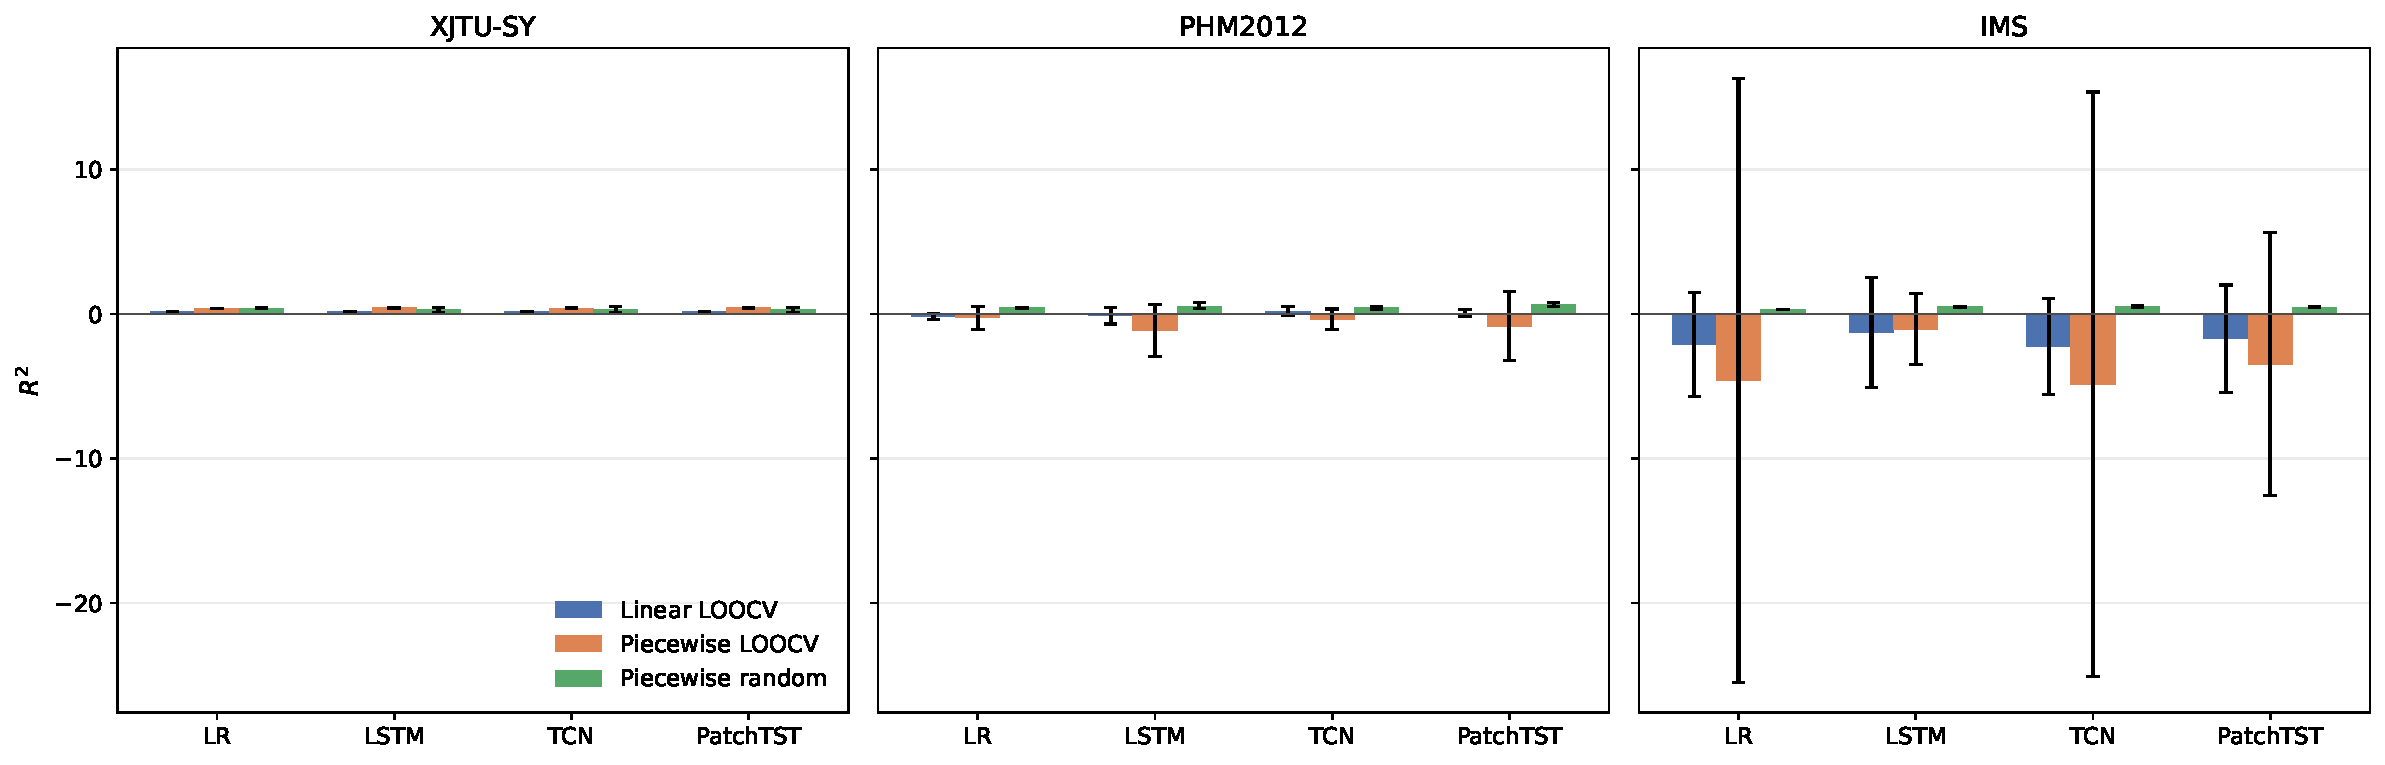
\includegraphics[width=0.92\textwidth]{figures/converged_r2_comparison_nonoverlap.pdf}
\caption{Non-overlap protocol comparison. The piecewise-random protocol raises mean $R^2$ above linear-LOOCV results, with dataset-dependent separation. Error bars show 95\% confidence intervals for LOOCV and observed min--max ranges for random splits.}
\label{fig:r2_nonoverlap}
\end{figure}

\begin{figure}[t]
\centering
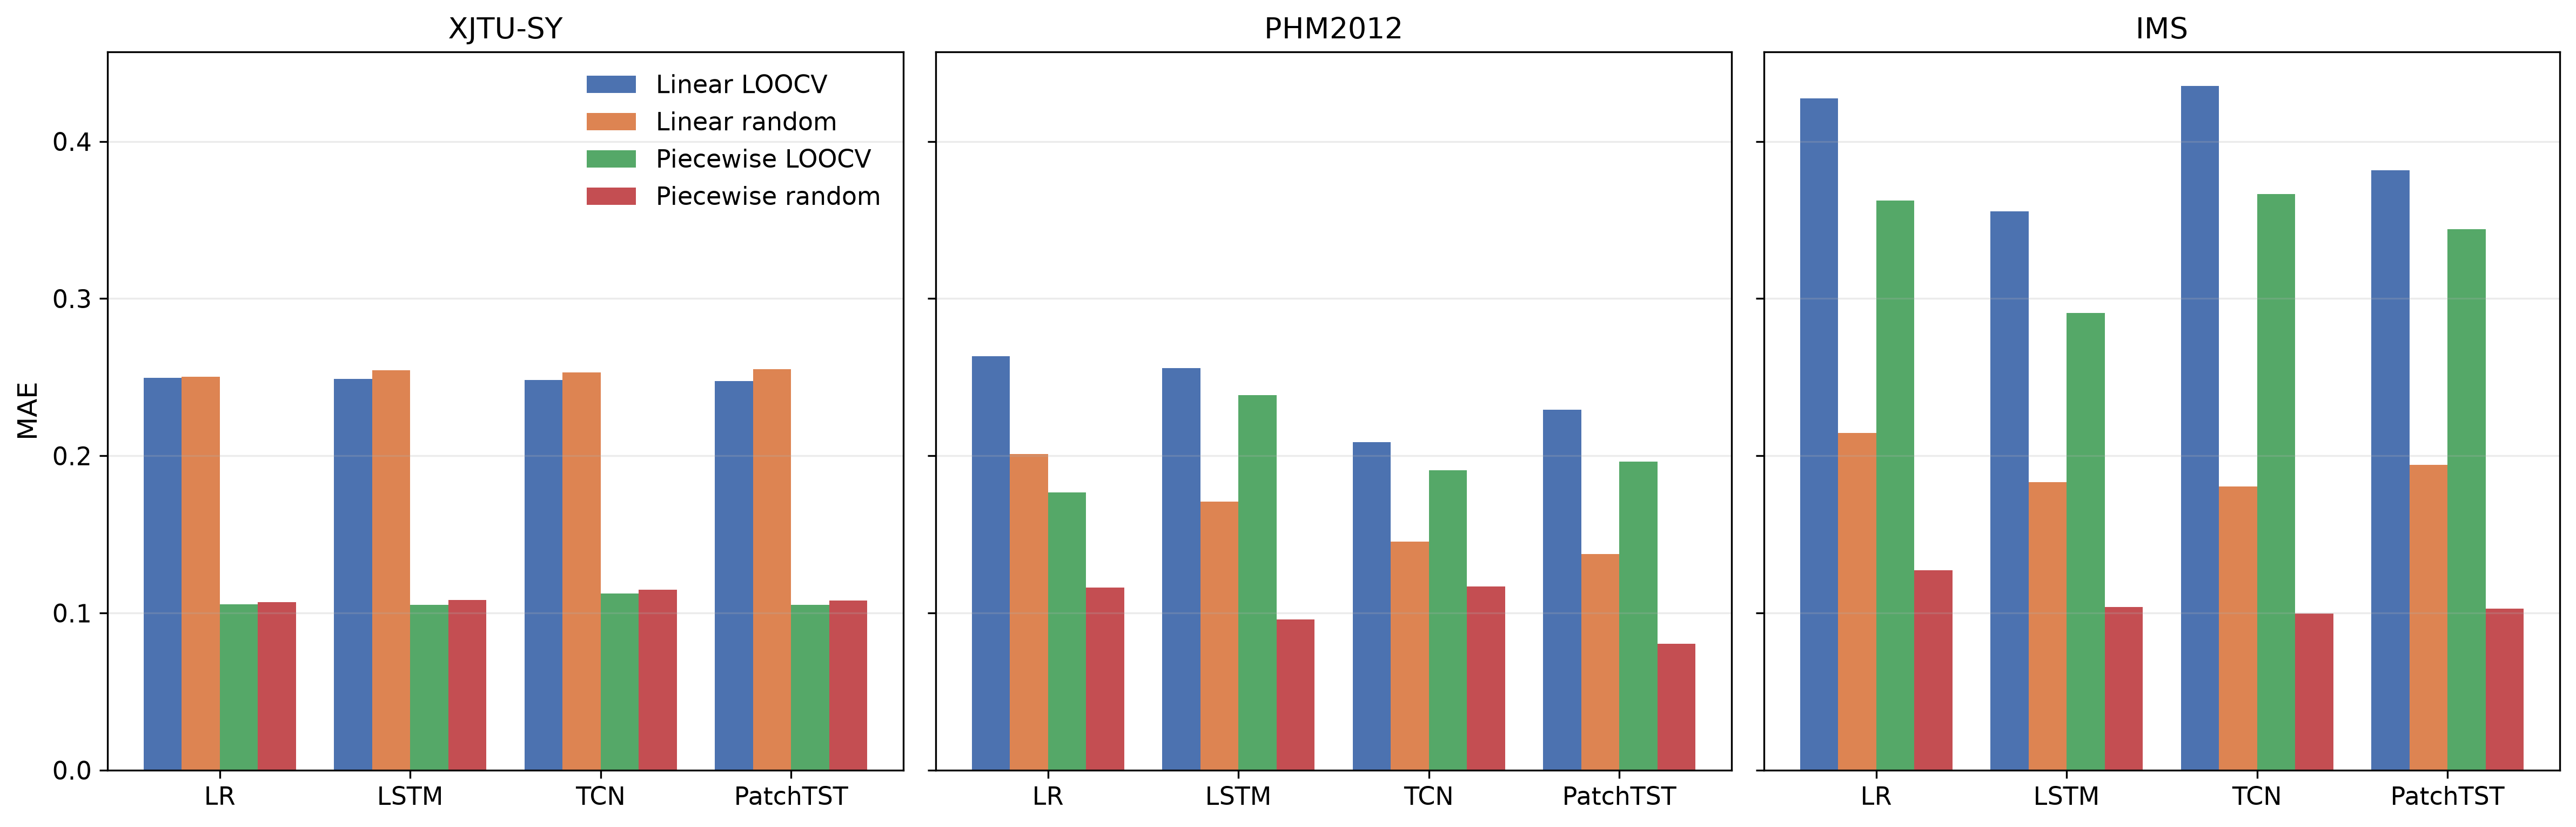
\includegraphics[width=0.9\textwidth]{figures/comparison_mae.png}
\caption{Complete $2\times2$ MAE comparison under the non-overlapping protocol. Lower MAE values indicate smaller prediction deviation on trajectory-normalized RUL.}
\label{fig:mae}
\end{figure}

\subsection{Constant Baseline and Cross-Bearing Generalization}
Table~\ref{tab:constant_baseline_nonoverlap} reports the constant predictor that always outputs the mean training RUL. Its $R^2$ is approximately zero in every dataset and label cell, while its RMSE and MAE provide the deployment-relevant floor. Several linear-LOOCV results have RMSE above this floor, especially on IMS, where a model must extrapolate across different test rigs and fault modes. This is not a numerical artifact: it shows that cross-bearing generalization is the real challenge. Random sequence-level splitting remains more favorable because test windows come from the same bearings and nearby temporal positions as training windows; dense overlapping history construction is associated with a larger apparent advantage.

\begin{table*}[!ht]
\centering
\caption{Constant predictor baseline under the non-overlapping stride-10 protocol. The constant predictor always outputs the mean training RUL. LOOCV values are mean [95\% CI]; random values are mean [min--max] across eight seeds.}
\label{tab:constant_baseline_nonoverlap}
\small
\resizebox{\textwidth}{!}{%
\begin{tabular}{lllccc}
\toprule
Dataset & Label & Protocol & $R^2$ & RMSE & MAE \\
\midrule
\midrule
XJTU-SY & linear & LOOCV & 0.000 & 0.289 & 0.250 \\
XJTU-SY & linear & Random & -0.001 [-0.003, 0.000] & 0.288 [0.284, 0.291] & 0.249 [0.245, 0.251] \\
\midrule
XJTU-SY & piecewise & LOOCV & 0.000 & 0.238 & 0.162 \\
XJTU-SY & piecewise & Random & -0.001 [-0.005, 0.000] & 0.240 [0.228, 0.256] & 0.163 [0.157, 0.171] \\
\midrule
PHM2012 & linear & LOOCV & 0.000 [0.000, 0.000] & 0.289 [0.289, 0.289] & 0.250 [0.250, 0.250] \\
PHM2012 & linear & Random & 0.000 [-0.001, 0.000] & 0.289 [0.286, 0.293] & 0.251 [0.247, 0.254] \\
\midrule
PHM2012 & piecewise & LOOCV & 0.000 [0.000, 0.000] & 0.239 [0.238, 0.239] & 0.162 [0.162, 0.163] \\
PHM2012 & piecewise & Random & -0.001 [-0.003, 0.000] & 0.243 [0.231, 0.256] & 0.165 [0.158, 0.172] \\
\midrule
IMS & linear & LOOCV & 0.000 [0.000, 0.000] & 0.289 [0.289, 0.289] & 0.250 [0.250, 0.250] \\
IMS & linear & Random & 0.000 [0.000, 0.000] & 0.289 [0.287, 0.291] & 0.250 [0.248, 0.253] \\
\midrule
IMS & piecewise & LOOCV & 0.000 [0.000, 0.000] & 0.238 [0.238, 0.238] & 0.162 [0.162, 0.162] \\
IMS & piecewise & Random & 0.000 [0.000, 0.000] & 0.239 [0.237, 0.243] & 0.163 [0.161, 0.165] \\
\bottomrule
\end{tabular}}
\end{table*}


\subsection{Split Sensitivity Results}
Table~\ref{tab:sensitivity_nonoverlap} reports TCN results under piecewise labels for the two additional random ratios and the chronological time-block split. The random-ratio results remain positive and are in the same general range as the main 70/15/15 result. In contrast, chronological time-block splitting produces large negative $R^2$ on all three datasets. The contrast indicates that the random-split advantage is not an artifact of one particular random ratio. The negative chronological results should not be read as a pure leakage effect because temporal extrapolation and degradation-stage imbalance also contribute.

\begin{table}[!ht]
\centering
\caption{TCN split sensitivity with non-overlap and piecewise labels. Random rows are mean [min--max] over seeds 42, 43, 44; time-block uses chronological 70/15/15 per bearing.}
\label{tab:sensitivity_nonoverlap}
\small
\begin{tabular}{llc}
\toprule
Dataset & Split & $R^2$ \\
\midrule
\midrule
XJTU-SY & Random 60/20/20 & 0.251 [0.106, 0.375] \\
XJTU-SY & Random 80/10/10 & 0.310 [0.043, 0.523] \\
XJTU-SY & Time-block 70/15/15 & -6.689 [-6.689, -6.689] \\
\midrule
PHM2012 & Random 60/20/20 & 0.435 [0.374, 0.471] \\
PHM2012 & Random 80/10/10 & 0.385 [0.337, 0.429] \\
PHM2012 & Time-block 70/15/15 & -6.883 [-6.883, -6.883] \\
\midrule
IMS & Random 60/20/20 & 0.502 [0.464, 0.552] \\
IMS & Random 80/10/10 & 0.508 [0.493, 0.526] \\
IMS & Time-block 70/15/15 & -7.650 [-7.650, -7.650] \\
\bottomrule
\end{tabular}
\end{table}



\subsection{Normalization and Validation-Bearing Sensitivity}
The primary evidence in this study is the non-overlapping history intervention, but two sensitivity checks bound the main interpretation. Table~\ref{tab:validation_sensitivity_nonoverlap} reports PHM2012 TCN linear-label LOOCV under validation-bearing offsets 1--5. The mean $R^2$ ranges from $-0.083$ to $0.040$, indicating that the fixed validation-bearing rule can affect cross-bearing estimates. The offset-1 row is a separate converged sensitivity run and is not the same designated main-table run, so small numerical differences from Table~\ref{tab:main_nonoverlap} are expected under GPU nondeterminism.

Table~\ref{tab:global_normalization_nonoverlap} reports PHM2012 TCN with globally normalized RUL targets. For linear labels, global normalization raises the random-split mean $R^2$ from $0.557$ (trajectory-normalized) to $0.729$ and makes linear LOOCV substantially worse. For piecewise labels, the random-split result remains close to the trajectory-normalized value. Normalization is therefore a protocol-dependent factor, especially for continuous labels, rather than a universal explanation of the split effect.

\begin{table}[!ht]
\centering
\caption{Validation-bearing sensitivity for PHM2012 TCN under the non-overlapping stride-10 protocol and linear labels. The main LOOCV protocol uses offset 1. Values are means across the six held-out bearings.}
\label{tab:validation_sensitivity_nonoverlap}
\small
\begin{tabular}{lccccc}
\toprule
Validation offset & $R^2$ mean & $R^2$ min--max & RMSE mean & MAE mean \\
\midrule
1 & 0.032 & -0.228--0.665 & 0.278 & 0.234 \\
2 & 0.018 & -0.376--0.755 & 0.277 & 0.230 \\
3 & -0.078 & -0.519--0.353 & 0.296 & 0.247 \\
4 & 0.040 & -0.714--0.557 & 0.273 & 0.233 \\
5 & -0.083 & -0.411--0.484 & 0.296 & 0.252 \\
\bottomrule
\end{tabular}
\end{table}


\begin{table}[!ht]
\centering
\caption{Global-normalization sensitivity for PHM2012 TCN under the non-overlapping stride-10 protocol. Random values are mean [min--max] across eight seeds (42--49).}
\label{tab:global_normalization_nonoverlap}
\small
\begin{tabular}{llcc}
\toprule
Label & LOOCV $R^2$ & Random $R^2$ & Random RMSE \\
\midrule
linear global & -3.807 [-12.404, 4.790] & 0.729 [0.657, 0.783] & 0.135 \\
piecewise global & -0.382 [-1.110, 0.346] & 0.424 [0.287, 0.549] & 0.185 \\
\bottomrule
\end{tabular}
\end{table}


\subsection{Protocol-Induced Differences and Their Boundary}
We evaluated the protocol family often used in recent bearing RUL benchmarks: piecewise 80\% plateau labels, random sequence-level splitting, converged deep training, and standard statistical features. Under overlapping stride~1 sequences, deep models reached $R^2$ values of $0.70$--$0.86$ on PHM2012 and IMS. Under non-overlapping stride~10 sequences, the same protocol reaches roughly $0.31$--$0.64$ across the deep models, still above the linear-LOOCV values but with substantially smaller margins.

We do not reproduce $R^2>0.99$. The protocol-level differences are reproducible, but the magnitude in our reproduced protocol family does not reach the near-perfect range reported by some papers. Public code and checkpoints were not available in our environment for the cited papers, so exact reproduction is not possible. We therefore do not claim that all published near-perfect values are explained by evaluation design. Our results are consistent with the view that dense overlapping history construction and within-trajectory dependence can raise scores for a within-trajectory interpolation task; they do not by themselves show that a model would generalize to a held-out bearing.

\section{Discussion}
\subsection{Random Splitting Measures Within-Trajectory Interpolation}
Tracking a known bearing and diagnosing a new asset call for different evidence. Consecutive windows from one bearing are strongly autocorrelated. A random split places test windows from the same trajectory in the training set, so the model can exploit nearby temporal context. Under LOOCV, the test bearing is completely absent during training. The large differences on PHM2012 and IMS show that reported performance is sensitive to how temporal history is sampled and partitioned. They do not justify a claim that model capacity plays no role, because training data composition and quantity also differ between protocols.
We therefore treat random splitting as measuring a different prediction task, not as an invalid protocol; its higher scores are informative for trajectory tracking but not evidence of held-out-bearing generalization.

\subsection{Trajectory-Normalized Cross-Bearing Evaluation}
In LOOCV, the held-out test bearing is absent from both training and validation. The protocol therefore answers a different question from random splitting: whether a model can generalize to a bearing trajectory that was not observed at the feature-window level. Because the current labels are normalized within each trajectory, this is a trajectory-normalized cross-bearing evaluation and measures relative degradation-position prediction rather than deployment to a new asset with unknown end of life. Several linear-LOOCV results fall below the constant baseline, especially on IMS. This is not a numerical artifact. The model is sometimes worse than predicting the mean when it must leave the training trajectory.
Extreme negative $R^2$ values on IMS should not be interpreted as evidence that the models are universally unusable; they indicate poor cross-bearing extrapolation under this particular feature/label pipeline, with only three held-out test sets.

\subsection{Chronological Splitting Measures Temporal Extrapolation}
Chronological splitting keeps the test bearing in training but evaluates later stages of the same trajectory. The negative $R^2$ values in Table~\ref{tab:sensitivity_nonoverlap} reflect temporal extrapolation and degradation-stage imbalance as well as the absence of random interleaving. The comparison is still useful because it shows that, under the same non-overlapping history construction, random sequence-level splitting rather than chronological ordering is what raises the scores on the same data.

Piecewise labels matter for a second reason: the 80\% plateau makes the label almost constant for most of life. On XJTU-SY, this improves apparent regression performance because the model only needs to recognize the transition region. On PHM2012 and IMS, the plateau can also interact with distribution shift and produce poor LOOCV results. The two practices should be reported separately, not combined into a single optimistic-bias multiplier.
\subsection{Label Construction Changes Target Difficulty}

Although $R^2$ reflects explained variance, MAE and RMSE quantify absolute prediction deviations. Table~\ref{tab:errors_nonoverlap} confirms that the primary protocol comparison is not an artifact of the $R^2$ scale: the piecewise-random protocol yields lower RMSE and MAE than the linear-LOOCV protocol across all three datasets.

\subsection{Implications for Bearing RUL Benchmarks}
For benchmark reporting, $R^2$ values are not comparable unless the split, label, and history-construction protocols are specified. The complete $2 \times 2$ protocol comparison in Table~\ref{tab:factorial_nonoverlap} summarizes label, split, and interaction effects more cleanly than a single protocol comparison; the stride intervention remains a separate history-construction analysis. MAE and RMSE should accompany $R^2$; a negative $R^2$ under distribution shift can otherwise obscure whether absolute error is actually large.

\subsection{Implications for Predictive Maintenance Deployment}
Benchmark scores are often used to assess deployment readiness, select models, set intervention thresholds, and plan maintenance windows. If the evaluation protocol permits within-trajectory interpolation, a high score may not transfer to a new asset or a changed operating condition. The result can be overconfident deployment, inappropriate maintenance timing, or excessive intervention. The STAR template treats evaluation protocol as part of deployment-reliability assessment rather than as a purely methodological detail.

For example, an enterprise selecting a model for a new production line may rely on a random-split benchmark and choose a model with a high reported $R^2$; under cross-bearing LOOCV on the same public data, the same model can fall below the constant baseline. Maintenance intervals planned from the optimistic score could lead to inappropriate maintenance timing, such as interventions scheduled too late or too early, and may contribute to unplanned downtime, spare-parts inventory pressure, or intervention cost. In manufacturing practice, the directly evaluated scenario is commissioning or monitoring a new bearing whose trajectory was not part of the training population. Changed operating conditions and machine-station transfer are not directly tested here. A random-split score answers whether the model can interpolate the already observed degradation of the same bearings; a cross-bearing score answers whether the model can support decisions before the new asset has accumulated a long history. STAR therefore provides a practical way to distinguish these two use cases during model selection and deployment review.

Table~\ref{tab:deployment_selection_nonoverlap} illustrates the model-selection consequence with actual non-overlap results. Under a random-split benchmark, PHM2012 PatchTST and IMS TCN are the stronger choices among the displayed models; under linear LOOCV, PHM2012 PatchTST remains the best displayed model while TCN drops sharply. On IMS, random-split scores remain positive while linear LOOCV is negative for every model. A deployment-oriented evaluation can therefore change model selection and, consequently, the confidence placed in maintenance decisions.


\begin{table}[!ht]
\centering
\caption{Illustrative protocol-dependent model-selection results under non-overlap. Random split uses piecewise labels; LOOCV uses linear labels.}
\label{tab:deployment_selection_nonoverlap}
\small
\begin{tabular}{llcc}
\toprule
Dataset & Model & Piecewise random $R^2$ & Linear LOOCV $R^2$ \\
\midrule
PHM2012 & TCN & 0.424 & 0.196 \\
PHM2012 & PatchTST & 0.642 & 0.059 \\
IMS & TCN & 0.522 & -2.230 \\
IMS & PatchTST & 0.469 & -1.721 \\
\bottomrule
\end{tabular}
\end{table}


\subsection{What Does a High $R^2$ Measure?}
A high $R^2$ under overlapping random sequence-level splitting may indicate interpolation aided by shared input content rather than cross-bearing predictive ability. The model can rely on adjacent windows from the same trajectory, on shared input content when stride~1 sequences are used, and on the monotonic structure of the label. This kind of performance is useful for tracking a known degradation process, but it does not show that the model can handle a new bearing, a different sensor position, or a different operating regime.

The distinction is visible in the LOOCV results: several models fall below the constant baseline on IMS, while the same models reach higher $R^2$ under random splitting.


\subsection{Positioning and Generalizability of the Benchmark Evidence}
The experiments use publicly available accelerated run-to-failure test beds rather than proprietary field data. The scope is limited to public accelerated-life test beds. We test whether benchmark protocol choices change reliability estimates, not whether a model reaches production grade on a specific factory line. Field deployment introduces additional confounders such as load variation, sensor drift, maintenance history, and incomplete run-to-failure records, so field validation remains future work rather than a claim of this paper. For industrial readers, the practical implication is that a benchmark score without STAR-type protocol evidence is not sufficient to infer new-asset reliability; for reviewers, the checklist provides a low-cost structure for checking the evidence behind a reported score.

\subsection{Practical Reporting Workflow}
We frame this paper as an empirically grounded evaluation-protocol audit template rather than a new model ranking. The template makes the intended task, data-splitting constraints, target construction, baseline, and reporting completeness auditable in a single workflow.

A benchmark result is interpretable only when the following items are reported together:
\begin{enumerate}
    \item the intended task, either held-out-bearing generalization under the benchmark data or trajectory tracking;
    \item the split protocol, including whether the test bearing is present in training;
    \item the label construction and all plateau parameters;
    \item the constant or median predictor baseline; and
    \item per-fold results with CI, RMSE, and MAE in addition to $R^2$.
\end{enumerate}
The STAR template in the next subsection turns these items into a reusable reporting checklist.

\subsection{STAR Reporting Template}
We summarize the experimentally supported reporting choices into the STAR template, which stands for Split integrity, Target integrity, Anchor baseline, and Reporting completeness. In this paper these map to:
\begin{enumerate}
    \item \textbf{Continuous labels}: continuous labels as the primary target; plateau parameters should be justified if plateau labels are retained.
    \item \textbf{Leave-one-bearing-out cross-validation}: no training window from the test bearing, with per-fold reporting.
    \item \textbf{Constant predictor baseline}: report the constant-predictor baseline as a reference floor.
    \item \textbf{Multi-model reporting}: multiple complementary model classes so conclusions are not specific to the evaluated model family.
\end{enumerate}
An adaptive debiased label that shortens the plateau and smooths the transition remains a practical intermediate option for applications that need early-stage noise suppression. The current experiments suggest that fixing the split protocol is at least as important as fixing the label.

Table~\ref{tab:star} summarizes the template as a reporting checklist. The checklist is derived from the protocol differences and controls observed in this study rather than from generic best-practice recommendations. The experiments are the primary contribution; STAR is an operationalization of their reporting implications rather than an independently validated standard. STAR is a reporting template, not a scoring or certification system; it specifies a recommended reporting structure for deployment-oriented cross-bearing evaluation rather than an exhaustive reliability certification procedure. Appendix A applies the checklist to representative studies as illustrative reporting extraction; the purpose is to make reporting choices explicit, not to judge the validity of individual models or results.

\begin{table*}[t]
\centering
\caption{STAR reporting structure recommended for deployment-relevant cross-bearing evaluation.}
\label{tab:star}
\small
\resizebox{\textwidth}{!}{%
\begin{tabular}{lll}
\toprule
Component & Recommended cross-bearing reporting practice & Status in this study \\
\midrule
Split integrity & Test bearing absent from training and validation & Overlapping random history split does not satisfy; LOOCV satisfies \\
Target integrity & Continuous or explicitly justified label construction & Linear and piecewise labels compared separately \\
Anchor baseline & Constant predictor reported as floor & Included \\
Reporting completeness & Per-fold results, CI, RMSE, MAE, seeds & Included \\
\bottomrule
\end{tabular}}
\end{table*}

Table~\ref{tab:star_before_after} shows the contrast between conventional reporting patterns and the STAR recommendations. The comparison makes the template actionable: a reader can check each row against a submitted benchmark and see which part of the evaluation protocol is missing.

Uncertainty-aware reporting is a direct extension of the STAR checklist. Conformal prediction and quantile-regression methods \citep{mst2024cqr,icsrs2023splitconformal,phme2026conformal,eaai2025explainable} can provide prediction intervals, coverage, and calibration metrics, but these measures are interpretable only when computed under the same split and label constraints as point forecasts. STAR can treat interval coverage, interval width, calibration, and transfer-condition disclosure as part of Reporting completeness, while keeping the test-bearing information constraints unchanged. We keep the primary analysis on point forecasts because the protocol effects are substantial but dataset-dependent. Extending the same protocol decomposition to interval predictors, transfer-learning settings, and field datasets is a natural next step rather than a claim of the present experiments.

\begin{table*}[t]
\centering
\caption{Conventional reporting patterns versus STAR recommendations.}
\label{tab:star_before_after}
\small
\resizebox{\textwidth}{!}{%
\begin{tabular}{lll}
\toprule
Aspect & Conventional pattern & STAR recommendation \\
\midrule
Split & Overlapping random history split & Test bearing absent from training and validation \\
Target & Piecewise plateau without justification & Continuous or explicitly justified label \\
Baseline & Constant predictor often omitted & Constant predictor reported \\
Reporting & Final $R^2$ only & Per-fold, CI, RMSE, MAE, seeds \\
\bottomrule
\end{tabular}}
\end{table*}

\subsection{Limitations}
This is a laboratory benchmark methodology study based on public accelerated-life datasets; it does not include field data. We did not reproduce exact published checkpoints because public code was unavailable. IMS has only three held-out test sets, so its confidence intervals are wide; we therefore treat IMS as directional evidence. The external datasets use the same statistical feature pipeline rather than each paper's raw-signal preprocessing; the conclusions therefore concern the evaluated feature/model family and should not be interpreted as model-agnostic across arbitrary raw-signal architectures. PU is not used because it does not provide run-to-failure trajectories. Trajectory-specific RUL normalization is an offline benchmark construction assumption and should not be interpreted as an online deployment procedure; Section~5.5 reports the global-normalization sensitivity separately. Seed-level bootstrap intervals in Appendix~B quantify computational split sensitivity rather than bearing-level uncertainty, and GPU numerical libraries can produce small run-to-run differences. The stride~1 versus stride~10 intervention changes overlap, sequence count, and temporal sampling density simultaneously, so the reported differences should be interpreted as a combined history-construction effect rather than as overlap alone. We do not claim a quantitative prevalence survey; the conclusions concern a commonly used protocol family rather than an assessment of individual papers. Appendix A demonstrates how the STAR checklist can support transparent reporting extraction. Future work should run exact published pipelines when code becomes available and extend STAR to raw-signal models, uncertainty-aware interval predictors, transfer-learning settings, and field datasets when they can be shared.

\section{Conclusion}
Using converged training on XJTU-SY, PHM2012, and IMS, we show that replacing dense overlapping history construction with non-overlapping stride-10 sequences reduced random-split $R^2$ in all 18 deep-model cells and increased RMSE and MAE in all 18 cells, while the linear-regression baseline, which uses single-window features, was unaffected. Because this intervention also changes sequence count and temporal sampling density, the result provides evidence that dense overlapping history construction can inflate apparent random-split performance relative to a non-overlapping stride-10 construction, rather than isolating overlap as the sole causal factor. The primary piecewise-random protocol still produced higher mean $R^2$ than the linear-label LOOCV reference across the three datasets, but the magnitude and statistical separation of this effect varied substantially across datasets, labels, and models. These protocol-induced differences are reproducible within our protocol family but do not reach or explain published near-perfect values; exact reproduction of original pipelines remains necessary. The STAR reporting template provides a recommended reporting structure for deployment-relevant cross-bearing evaluation, supporting model selection and review. The contribution is a reusable empirically grounded evaluation-protocol audit template that quantifies protocol-induced reliability differences and shows that temporal history construction is itself an important source of evaluation sensitivity in RUL prediction.

\appendix
\section*{Appendix A. Illustrative Examples of Reporting Extraction}
To support transparent reporting without judging individual studies, the STAR checklist can be recorded as \emph{reported}, \emph{unclear}, or \emph{unavailable}. \emph{Reported} means that the item is explicitly described in the examined full text; \emph{unclear} means that the description is incomplete or ambiguous; \emph{unavailable} means that the information could not be verified from the examined source. The checklist records what is reported, not whether a study is valid.

Table~\ref{tab:star_audit} illustrates how reporting choices can be extracted from five examples whose full texts are publicly available from their journals. The coding sheet uses the same three-level vocabulary for candidate studies; rows should be completed only after full-text examination.

\begin{table*}[t]
\centering
\caption{Illustrative examples of reporting extraction. Entries record what can be verified from the examined full texts and are not correctness judgments.}
\label{tab:star_audit}
\small
\resizebox{\textwidth}{!}{%
\begin{tabular}{llllll}
\toprule
Study & Dataset & Split & Target construction & Anchor baseline & Reporting completeness \\
\midrule
\citet{wu2020cascade} & PHM2012 & Leave-one-bearing-out & Linear reliability rate & Unavailable & Unavailable \\
\citet{yang2024cnnvaembilstm} & Industrial weaving-machine case & Bearing-level 70/30 train/test & Normalized RUL (construction details unclear) & Unavailable & Data not public; no code \\
\citet{wen2024envelope} & XJTU-SY & Leave-one-bearing-out within condition & Piecewise linear RUL (plateau unclear) & Unavailable & Dataset available; no code \\
\citet{li2022twostage} & PHM2012 & Cross-condition bearing holdout & Health percentage after IF (pre-IF plateau) & Unavailable & Data on request; no code \\
\citet{li2022soasvm} & IMS & Within-trajectory parity 1:1 & PCA degradation index & Unavailable & Data in article; no code \\
\bottomrule
\end{tabular}}
\end{table*}

\backmatter

\bmhead{Supplementary information}
The v26 reproducibility snapshot is included with this submission and is available at \url{https://github.com/KKK-cell441/rul-evaluation-star/tree/v26-audit-snapshot}. It contains preprocessing scripts, converged training and split sensitivity runners for the non-overlapping stride~10 protocol, per-fold and per-seed JSON results, validation-bearing sensitivity, global-normalization sensitivity, table/figure generators, and no machine-specific absolute paths.

\clearpage
\section*{Appendix B. Per-Fold and Per-Seed Evidence}
\begin{table*}[!ht]
\centering
\caption{Per-fold and per-seed evidence for the non-overlap primary protocol comparison. LOOCV range is the min--max of linear-label fold $R^2$; seed columns are piecewise-label random-split $R^2$ for seeds 42--49.}
\label{tab:perfold_nonoverlap}
\small
\resizebox{\textwidth}{!}{%
\begin{tabular}{lllccccccccc}
\toprule
Dataset & Model & Linear LOOCV range & S42 & S43 & S44 & S45 & S46 & S47 & S48 & S49 & Protocol gap \\
\midrule
XJTU-SY & Linear Reg. & $0.176$ to $0.181$ & 0.447 & 0.414 & 0.429 & 0.364 & 0.400 & 0.416 & 0.399 & 0.375 & 0.228 \\
XJTU-SY & LSTM & $0.192$ to $0.195$ & 0.073 & 0.353 & 0.447 & 0.164 & 0.322 & 0.443 & 0.428 & 0.253 & 0.117 \\
XJTU-SY & TCN & $0.188$ to $0.192$ & 0.123 & 0.316 & 0.501 & 0.161 & 0.356 & 0.440 & 0.453 & 0.287 & 0.140 \\
XJTU-SY & PatchTST & $0.194$ to $0.197$ & 0.075 & 0.338 & 0.462 & 0.168 & 0.315 & 0.431 & 0.457 & 0.269 & 0.118 \\
PHM2012 & Linear Reg. & $-0.444$ to $0.101$ & 0.376 & 0.396 & 0.420 & 0.435 & 0.426 & 0.465 & 0.424 & 0.385 & 0.584 \\
PHM2012 & LSTM & $-0.822$ to $0.419$ & 0.606 & 0.477 & 0.567 & 0.600 & 0.364 & 0.372 & 0.357 & 0.806 & 0.637 \\
PHM2012 & TCN & $-0.245$ to $0.502$ & 0.548 & 0.444 & 0.418 & 0.378 & 0.366 & 0.286 & 0.512 & 0.437 & 0.227 \\
PHM2012 & PatchTST & $-0.134$ to $0.539$ & 0.790 & 0.573 & 0.709 & 0.681 & 0.511 & 0.509 & 0.628 & 0.734 & 0.583 \\
IMS & Linear Reg. & $-3.000$ to $-0.452$ & 0.328 & 0.313 & 0.318 & 0.333 & 0.315 & 0.310 & 0.327 & 0.319 & 2.429 \\
IMS & LSTM & $-2.956$ to $0.022$ & 0.506 & 0.458 & 0.465 & 0.484 & 0.507 & 0.465 & 0.452 & 0.542 & 1.764 \\
IMS & TCN & $-3.006$ to $-0.685$ & 0.566 & 0.502 & 0.487 & 0.529 & 0.540 & 0.484 & 0.500 & 0.571 & 2.752 \\
IMS & PatchTST & $-2.741$ to $0.001$ & 0.507 & 0.442 & 0.466 & 0.471 & 0.482 & 0.448 & 0.423 & 0.517 & 2.190 \\
\bottomrule
\end{tabular}}
\end{table*}


\begin{table*}[!ht]
\centering
\caption{Seed-level bootstrap summaries for random sequence-level splitting under the non-overlapping stride-10 protocol. Bootstrap intervals resample the eight fixed seed runs and quantify computational split sensitivity, not independent bearing-level uncertainty.}
\label{tab:random_bootstrap_nonoverlap}
\small
\resizebox{\textwidth}{!}{%
\begin{tabular}{lllccccc}
\toprule
Dataset & Model & Label & $R^2$ mean [95\% CI] & RMSE mean [95\% CI] & MAE mean [95\% CI] \\
\midrule
XJTU-SY & Linear Reg. & linear & 0.165 [0.157, 0.174] & 0.263 [0.262, 0.264] & 0.250 [0.250, 0.251] \\
XJTU-SY & LSTM & linear & 0.117 [0.073, 0.159] & 0.267 [0.263, 0.272] & 0.254 [0.251, 0.258] \\
XJTU-SY & TCN & linear & 0.124 [0.075, 0.173] & 0.266 [0.261, 0.271] & 0.253 [0.249, 0.257] \\
XJTU-SY & PatchTST & linear & 0.095 [0.050, 0.139] & 0.271 [0.266, 0.275] & 0.255 [0.252, 0.258] \\
XJTU-SY & Linear Reg. & piecewise & 0.405 [0.388, 0.423] & 0.185 [0.183, 0.187] & 0.107 [0.105, 0.109] \\
XJTU-SY & LSTM & piecewise & 0.310 [0.218, 0.393] & 0.190 [0.186, 0.195] & 0.108 [0.103, 0.114] \\
XJTU-SY & TCN & piecewise & 0.330 [0.242, 0.415] & 0.187 [0.183, 0.191] & 0.115 [0.109, 0.121] \\
XJTU-SY & PatchTST & piecewise & 0.314 [0.221, 0.399] & 0.189 [0.186, 0.193] & 0.108 [0.102, 0.112] \\
PHM2012 & Linear Reg. & linear & 0.282 [0.270, 0.295] & 0.245 [0.243, 0.247] & 0.201 [0.199, 0.203] \\
PHM2012 & LSTM & linear & 0.455 [0.412, 0.504] & 0.215 [0.203, 0.225] & 0.171 [0.156, 0.184] \\
PHM2012 & TCN & linear & 0.557 [0.543, 0.573] & 0.194 [0.190, 0.198] & 0.145 [0.141, 0.149] \\
PHM2012 & PatchTST & linear & 0.616 [0.589, 0.641] & 0.180 [0.173, 0.188] & 0.137 [0.130, 0.144] \\
PHM2012 & Linear Reg. & piecewise & 0.416 [0.397, 0.435] & 0.186 [0.183, 0.189] & 0.116 [0.114, 0.118] \\
PHM2012 & LSTM & piecewise & 0.518 [0.422, 0.620] & 0.168 [0.150, 0.183] & 0.096 [0.087, 0.104] \\
PHM2012 & TCN & piecewise & 0.424 [0.370, 0.477] & 0.186 [0.179, 0.193] & 0.117 [0.112, 0.122] \\
PHM2012 & PatchTST & piecewise & 0.642 [0.574, 0.708] & 0.145 [0.134, 0.157] & 0.080 [0.077, 0.084] \\
IMS & Linear Reg. & linear & 0.218 [0.214, 0.221] & 0.256 [0.255, 0.257] & 0.215 [0.214, 0.216] \\
IMS & LSTM & linear & 0.382 [0.364, 0.400] & 0.228 [0.223, 0.231] & 0.183 [0.179, 0.186] \\
IMS & TCN & linear & 0.395 [0.380, 0.414] & 0.225 [0.220, 0.229] & 0.180 [0.176, 0.184] \\
IMS & PatchTST & linear & 0.331 [0.312, 0.353] & 0.237 [0.232, 0.241] & 0.194 [0.191, 0.197] \\
IMS & Linear Reg. & piecewise & 0.320 [0.315, 0.326] & 0.197 [0.196, 0.198] & 0.127 [0.127, 0.128] \\
IMS & LSTM & piecewise & 0.485 [0.466, 0.506] & 0.171 [0.166, 0.176] & 0.104 [0.100, 0.108] \\
IMS & TCN & piecewise & 0.522 [0.501, 0.544] & 0.164 [0.160, 0.169] & 0.100 [0.096, 0.104] \\
IMS & PatchTST & piecewise & 0.469 [0.449, 0.490] & 0.173 [0.168, 0.179] & 0.103 [0.099, 0.107] \\
\bottomrule
\end{tabular}}
\end{table*}


\section*{Declarations}
\begin{itemize}
\item Funding: This research received no specific grant from any funding agency in the public, commercial, or not-for-profit sectors.
\item Conflict of interest: The authors declare that they have no known competing financial interests or personal relationships that could have appeared to influence the work reported in this paper.
\item Ethics approval and consent to participate: Not applicable.
\item Consent for publication: Not applicable.
\item Data availability: The XJTU-SY, PHM2012, and IMS datasets are publicly available from their original sources.
\item Code availability: The v26 reproducibility snapshot is available at \url{https://github.com/KKK-cell441/rul-evaluation-star/tree/v26-audit-snapshot}. The maintained Zenodo record \url{https://doi.org/10.5281/zenodo.21887653} will be updated to this snapshot before the final version of record.
\item Author contribution: Zhongkuan Ma: Conceptualization, Methodology, Software, Validation, Formal analysis, Writing - Original Draft, Writing - Review \& Editing.
\item ORCID: 0009-0003-4491-6619.
\end{itemize}

\begin{thebibliography}{99}

\bibitem[Caesarendra and Tjahjowidodo(2021)]{caesarendra2021machine}
W. Caesarendra and T. Tjahjowidodo,
``Machine learning methods for bearing fault diagnosis: A comprehensive review,''
\textit{Mech. Syst. Signal Process.}, vol.~152, p.~107397, 2021.

\bibitem[Hughes and Zhang(2026)]{leakage_frontiers}
C. M. L. Hughes and Y. Zhang,
``Bursting the bubble: Data leakage and inflated deep learning accuracy in multivariate time-series frailty classification,''
\textit{Front. Comput. Sci.}, vol.~8, p.~1700489, 2026. doi:10.3389/fcomp.2026.1700489.

\bibitem[Ince et al.(2016)]{ince2016real}
T. Ince, S. Kiranyaz, L. Eren, M. Askar, and M. Gabbouj,
``Real-time motor fault detection by 1-D convolutional neural networks,''
\textit{IEEE Trans. Ind. Electron.}, vol.~63, no.~11, pp.~7067--7075, 2016.

\bibitem[Kotzalas and Harris(2004)]{kotzalas2004fatigue}
M. N. Kotzalas and T. A. Harris,
``Fatigue failure and life prediction of rolling bearings,''
\textit{Tribol. Trans.}, vol.~47, no.~3, pp.~409--418, 2004.

\bibitem[Lei et al.(2018)]{lei2018machinery}
Y. Lei, N. Li, L. Guo, N. Li, T. Yan, and J. Lin,
``Machinery health prognostics: A systematic review from data acquisition to RUL prediction,''
\textit{Mech. Syst. Signal Process.}, vol.~104, pp.~799--834, 2018.

\bibitem[Li et al.(2022a)]{li2022physics}
T. Li, Z. Zhou, S. Li, and Y. Chen,
``Physics-informed neural networks for bearing remaining useful life prediction,''
\textit{Reliab. Eng. Syst. Saf.}, vol.~224, p.~108548, 2022.

\bibitem[Li et al.(2022b)]{li2022twostage}
X. Li, K. Zhang, W. Li, Y. Feng, and R. Liu,
``A two-stage transfer regression convolutional neural network for bearing remaining useful life prediction,''
\textit{Machines}, vol.~10, no.~5, p.~369, 2022. doi:10.3390/machines10050369.

\bibitem[Li et al.(2022c)]{li2022soasvm}
X. Li, S. An, Y. Shi, and Y. Huang,
``Remaining useful life estimation of rolling bearing based on SOA-SVM algorithm,''
\textit{Machines}, vol.~10, no.~9, p.~729, 2022. doi:10.3390/machines10090729.

\bibitem[Liu et al.(2021)]{reg_lstm_2021}
Z.-H. Liu, X.-D. Meng, H.-L. Wei, L. Chen, B.-L. Lu, Z.-H. Wang, and L. Chen,
``A regularized LSTM method for predicting remaining useful life of rolling bearings,''
\textit{Int. J. Autom. Comput.}, vol.~18, no.~4, pp.~581--593, 2021. doi:10.1007/s11633-020-1276-6.

\bibitem[Mao et al.(2024)]{mst2024cqr}
S. Mao, X. Li, and B. Zhao,
``Remaining useful life prediction based on time-series features and conformalized quantile regression,'' \textit{Meas. Sci. Technol.}, vol.~35, 2024. doi:10.1088/1361-6501/ad762c.

\bibitem[Nectoux et al.(2012)]{nectoux2012pronostia}
P. Nectoux, R. Gouriveau, K. Medjaher, E. Ramasso, B. Chebel-Morello, N. Zerhouni, and C. Varnier,
``PRONOSTIA: An experimental platform for bearings accelerated degradation tests,''
in \textit{IEEE Int. Conf. Prognostics and Health Management}, 2012, pp.~1--8.

\bibitem[Nie et al.(2023)]{patchtst2023}
Y. Nie, N. H. Nguyen, P. Sinthong, and J. Kalagnanam,
``A time series is worth 64 words: Long-term forecasting with transformers,''
in \textit{Proc. Int. Conf. Learn. Represent.}, 2023.

\bibitem[Paris and Erdogan(1963)]{paris1963critical}
P. Paris and F. Erdogan,
``A critical analysis of crack propagation laws,''
\textit{J. Basic Eng.}, vol.~85, no.~4, pp.~528--534, 1963.

\bibitem[Peng et al.(2023)]{transformer_tim_2023}
H. Peng, B. Jiang, Z. Mao, and S. Liu,
``Local enhancing transformer with temporal convolutional attention mechanism for bearings remaining useful life prediction,''
\textit{IEEE Trans. Instrum. Meas.}, vol.~72, pp.~1--12, 2023. doi:10.1109/tim.2023.3291787.

\bibitem[Qiu et al.(2006)]{ims2006}
H. Qiu, J. Lee, J. Lin, and G. Yu,
``Wavelet filter-based weak signature detection method and its application on rolling element bearing prognostics,''
\textit{J. Sound Vib.}, vol.~289, no.~4--5, pp.~1066--1090, 2006.

\bibitem[Que et al.(2021)]{gru_tim_2021}
Z. Que, X. Jin, and Z. Xu,
``Remaining useful life prediction for bearings based on a gated recurrent unit,''
\textit{IEEE Trans. Instrum. Meas.}, vol.~70, pp.~1--11, 2021. doi:10.1109/tim.2021.3054025.

\bibitem[Salinas-Camus et al.(2025)]{phmconf2025rethinking}
M. Salinas-Camus, K. Goebel, and N. Eleftheroglou,
``Rethinking RUL prediction,'' in \textit{Annu. Conf. PHM Soc.}, vol.~17, 2025. doi:10.36001/phmconf.2025.v17i1.4361.

\bibitem[Stock et al.(2023)]{leakage_nature}
A. Stock, E. J. Gregr, and K. M. A. Chan,
``Data leakage jeopardizes ecological applications of machine learning,''
\textit{Nat. Ecol. Evol.}, vol.~7, no.~11, pp.~1743--1745, 2023. doi:10.1038/s41559-023-02162-1.

\bibitem[Vaswani et al.(2017)]{vaswani2017attention}
A. Vaswani, N. Shazeer, N. Parmar, J. Uszkoreit, L. Jones, A. N. Gomez, L. Kaiser, and I. Polosukhin,
``Attention is all you need,''
in \textit{Proc. NeurIPS}, vol.~30, 2017.

\bibitem[Wang et al.(2019)]{xjtusy2019dataset}
B. Wang, Y. Lei, N. Li, and N. Li,
``XJTU-SY rolling element bearing accelerated life test dataset,''
\textit{Data in Brief}, vol.~25, p.~104122, 2019.

\bibitem[Wang et al.(2026)]{phme2026conformal}
S. Wang, Y. Vidal, and F. Pozo,
``Uncertainty-aware bearing remaining useful life prediction based on conformal prediction,'' in \textit{PHM Soc. Eur. Conf.}, vol.~9, 2026. doi:10.36001/phme.2026.v9i1.4902.

\bibitem[Wen et al.(2024)]{wen2024envelope}
H. Wen, L. Zhang, and J. K. Sinha,
``From envelope spectra to bearing remaining useful life: An intelligent vibration-based prediction model with quantified uncertainty,''
\textit{Sensors}, vol.~24, no.~22, p.~7257, 2024. doi:10.3390/s24227257.

\bibitem[Wu and Zhang(2020)]{wu2020cascade}
Q. Wu and C. Zhang,
``Cascade fusion convolutional long-short time memory network for remaining useful life prediction of rolling bearing,''
\textit{IEEE Access}, vol.~8, pp.~32957--32965, 2020. doi:10.1109/access.2020.2970444.

\bibitem[Xia et al.(2020)]{review2020bearing}
Z. Xia, Q. Guan, Y. Gao, X. Chen, and X. Zhai,
``Review on remaining useful life prediction methods of bearing,'' in \textit{Int. Conf. Prognostics and System Health Management}, 2020. doi:10.1109/PHM-Jinan48558.2020.00083.

\bibitem[Xu and Zio(2023)]{icsrs2023splitconformal}
W. Xu and E. Zio,
``A general data-driven framework for remaining useful life estimation with uncertainty quantification using split conformal prediction,'' in \textit{Int. Conf. Syst. Reliab. Saf.}, 2023. doi:10.1109/ICSRS59833.2023.10381131.

\bibitem[Yang et al.(2022)]{rul_lstm_uq_2022}
J. Yang, Y. Peng, J. Xie, and P. Wang,
``Remaining useful life prediction method for bearings based on LSTM with uncertainty quantification,''
\textit{Sensors}, vol.~22, no.~12, p.~4549, 2022. doi:10.3390/s22124549.

\bibitem[Yang et al.(2024)]{yang2024cnnvaembilstm}
L. Yang, Y. Jiang, K. Zeng, and T. Peng,
``Rolling bearing remaining useful life prediction based on CNN-VAE-MBiLSTM,''
\textit{Sensors}, vol.~24, no.~10, p.~2992, 2024. doi:10.3390/s24102992.

\bibitem[Zhang and Wang(2025)]{eaai2025explainable}
T. Zhang and H. Wang,
``Explainable remaining useful life uncertainty prediction method for rolling bearing,'' \textit{Eng. Appl. Artif. Intell.}, vol.~142, 2025. doi:10.1016/j.engappai.2025.112114.

\bibitem[Zhao et al.(2019)]{zhao2019deep}
R. Zhao, R. Yan, Z. Chen, K. Mao, P. Wang, and R. X. Gao,
``Deep learning and its applications to machine health monitoring,''
\textit{Mech. Syst. Signal Process.}, vol.~115, pp.~213--237, 2019.

\bibitem[Zhao et al.(2021)]{zhao2021deep}
M. Zhao, M. Kang, B. Tang, and M. Pecht,
``Deep learning for bearing prognostics: A comprehensive review,''
\textit{IEEE Trans. Rel.}, vol.~70, no.~4, pp.~1431--1451, 2021.

\bibitem[Zhu et al.(2022)]{ress2022bayesian}
R. Zhu, Y. Chen, W. Peng, and Z.-S. Ye,
``Bayesian deep-learning for RUL prediction: An active learning perspective,'' \textit{Reliab. Eng. Syst. Saf.}, vol.~228, 2022. doi:10.1016/j.ress.2022.108758.
\end{thebibliography}

\end{document}



